\newpage
\chapter{Proposed hardware implementation}
\label{sec:implementation}
The following chapter describes the proposed implementation of the ACAD anomaly detector on a Zynq Z-7030 or Z-7035 device, used by the NTNU Smallsat project. \\

\section{Memory considerations}
\label{sec:memory_management}
    As the ACAD anomaly detector is to be implemented on a Zynq Z-7030 or Z-7035 device, care must be taken when designing, with respect to logic and memory usage. The hyperspectral image data inputted to the AD might have number of spectral bands, $P\_bands$ = $N\_bands$, depending upon if preprocessing steps such as Principal Component Analysis (PCA) is done on the image cube. $Pixel\_data\_width$ is the width of the data per spectral band of the input pixel to the AD. This will be up to 16-bit in the SmallSat project. The large size of $P\_bands$ and $Pixel\_data\_width$ makes memory usage an important consideration.

\subsection{Storing and updating matrices in ACAD }
\label{sec:mem_management_correlation_matrix}
The ACAD algorithm requires storage of the following matrices: $\textbf{R(x}_k)$, $\Tilde{\textbf{R}}(\textbf{x}_k)$ and $\sum_{t_j\in\Delta(k)}\textbf{t}_j\textbf{t}_j^T$. In addition the matrix $A$ and $A^{-1}$ used in Gauss-Jordan elimination shown in Figure \ref{fig:matrix_A_and} must be stored in memory. These are $P\_bands$ $\times$ $P\_bands$ sized matrices. 

\begin{figure}[H]
\centering                                                              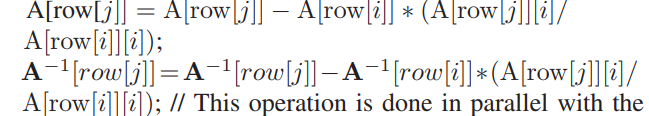
\includegraphics[scale=0.5]{images/matrix_A_and_inv.PNG}
  \caption{Matrix $A$ and $A^{-1}$ used in Gauss-Jordan elimination.} 
  \label{fig:matrix_A_and}.
\end{figure}

Storing and updating matrices of size $P\_bands$ $\times$ $P\_bands$  requires a lot of memory resources. %the causal correlation matrix sum as shown in equation \ref{eq:caus_corr} requires a lot of memory resources. 
One of the matrices is the causal correlation matrix $\textbf{R(x}_k)$. Update of this matrix needs to be done for each pixel in the image, and the memory used for this operation is therefore important in order to make the AD real-time.  As $\textbf{R(x}_k)$ is the product of $\textbf{x}$ $\times$ $\textbf{x}^T$ the resulting data width will be 2$\times$ $Pixel\_data\_width$. Using spectral information from all $N\_bands$ would require $P\_bands$ $\times$ $P\_bands$ $\times$ $32$ $=$ $100$ $\times$ $100$ $\times$ $32$ bit = $320 kbit$ of memory storage. 
\\

There are two alternatives to storing all this information on the FPGA; storing it in block RAM or in registers. The FPGA used in the SmallSat's first prototype is the Zynq Z-7030 or the Zynq Z-7035. 
The FPGAs contains the memory resources as shown in figure \ref{fig:zynq_memory_resources}. The Z-7030 and the Z-7035 contains 265 and 500 36kbit BRAM blocks respectively. The number of DSP Slices are 400 for the Z-7030 and 900 for the Z-7035. 





\begin{figure}[H]
\hbox{\hspace*{-1cm}                               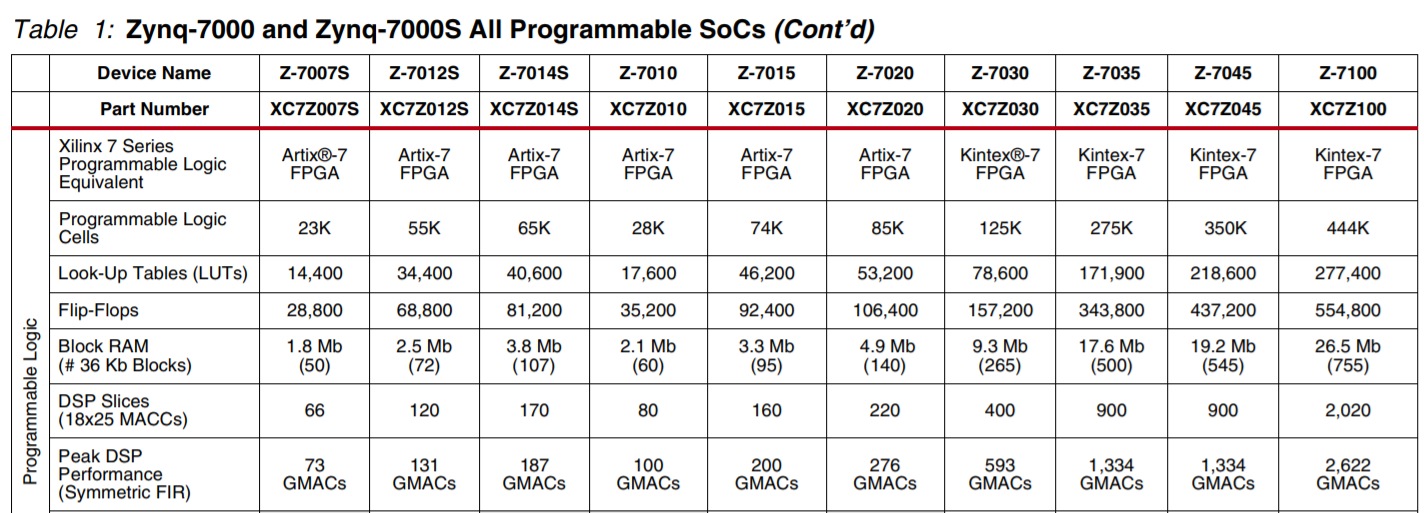
\includegraphics[scale=0.45]{images/zynq_memory_resources.PNG}}
  \caption{Zynq memory resources \cite{cite:mem_resources_zynq}.} 
  \label{fig:zynq_memory_resources}.
\end{figure}

\subsubsection{Using registers}
The Zynq Z-7030 and the Zynq Z-7035 contains $157,200$ and $343,800$ flip flops each, respectively. By using equation \ref{eq:max_bands}:%, the maximal number of spectral bands used is 70 and 103.
\begin{equation}
    max\_bands= \sqrt{\frac{number\_of\_registers}{2*pixel\_data\_width \times number\_of\_matrices}},
    \label{eq:max_bands}
\end{equation}

it is possible to do an estimation of the maximum value of $P\_bands$ if using registers for storage of the matrices. $number\_of\_matrices$ is the number of matrices of size $P\_bands$ $\times$ $P\_bands$ that needs to be stored in memory. For $number\_of\_matrices$=5, $max\_bands$ =[31, 46] for Z-7030 and Z-7035 respectively.


However, this is unrealistic as this leaves no flip flop free for other use in the design. As the AD implemented in this task is a part of a larger processing pipeline it is not acceptable to use all of the available flip flops. Assuming that it is acceptable to use 15\% of the available flip flops, the number of spectral bands that can be used is 12 and 17 for the Zynq Z-7030 and the Zynq Z-7035 respectively. Dimensional reduction to reduce $P\_bands$ from 100 to 12 or 17 can be done through pre-prossesing of data by for example PCA.
The benefit of the use of registers is the ability of instantaneous update. %This will lead to the AD becoming closer to real-time than if distributed RAM or BRAM is used.



\subsubsection{Using BRAM}
The Z-7030 and the Z-7035 contains 265 and 500 $36$kbit BRAM - blocks respectively. In  order to store the largest matrix of $320 kbit$ a minimum of 9 BRAM blocks are needed. Each 36 kbit BRAM block consists of two 18 kbit BRAM blocks. In true dual port (TDP) mode \cite{cite:ug953}, it is possible to do two writes and two reads per 36kbit BRAM per clock cycle, with each write and read being maximum 36 bits. BRAMs in TDP mode have only one address input, the same address for reads and writes. This makes it hard to use for the correlation module, as the ACAD correlation needs to read previously stored data from the BRAM before writing to the same address. Therefore, it is necessary to have a separate read and write address. By inferring two separate Simple Dual Port (SDP) 18kbit BRAMs, by the code shown in Listing \ref{lst:inferr_bram}, it is possible to get two writes and two reads per cycle, with separate read and write addresses.

\lstinputlisting[caption={Code for inferring a SDP 18 kbit BRAM.},label={lst:inferr_bram},style=customc]{code/bram_espen_sdp.vhd}







To be able to evaluate if it is possible to store a matrix of size $P\_bands$ $\times$ $P\_bands$ $Pixel\_data\_width$ $\times$ 2 in BRAM, with acceptably low time spent updating the matrix, the time spent updating $\Tilde{\textbf{R}}(\textbf{x}_k)$ has been used as a benchmark. Equation \ref{eq:clk_cycles_corr_update_BRAM} shows the calculation of number of clock cycles needed to update $\Tilde{\textbf{R}}(\textbf{x}_k)$ of size $P\_bands$ $\times$ $P\_bands$, $n\_clk\_update\_corr\_BRAM$: 

\begin{equation}
    n\_clk\_update\_corr\_BRAM = \frac{P\_bands \times P\_bands }{2 \times N\_bram\_correlation}.
    \label{eq:clk_cycles_corr_update_BRAM}
\end{equation}


The update is done for each pixel in the image. $N\_bram\_correlation$ is the number of 36 kbit BRAMs used to store $\Tilde{\textbf{R}}(\textbf{x}_k)$. The total time spent updating $\Tilde{\textbf{R}}(\textbf{x}_k)$ for the entire image is given by equation \ref{eq:clk_cycles_corr_image}:

\begin{equation}
    clk\_corr\_image\_BRAM = N\_pixels \times N\_rows \times n\_clk\_update\_corr\_BRAM.
    \label{eq:clk_cycles_corr_image}
\end{equation}

Updating a matrix with $P\_bands$ = 100, using 9 BRAMs would require 556 clk cycles. For the entire image, having $N\_pixels$ the total amount of clock cycles spent updating the correlation matrix would be 349648384. At a target clock frequency of 100 MHz this would require $3.49648$ seconds.





Figure \ref{fig:update_time_correlation_BRAM} shows the estimated total time spent updating $\Tilde{\textbf{R}}(\textbf{x}_k)$ for an image of $N\_rows$ =1088 $\times$ $N\_pixels$ = 578 , with a target clock frequency of 100 MHz. Plotted as a function of number of 36 kbit BRAMs used to store and update $\Tilde{\textbf{R}}(\textbf{x}_k)$. The BRAMs are assumed written to in parallel. Plotted for $P\_bands$ =[20, 30, 40, 50, 60, 70, 80, 90, 100].

\begin{figure}[H]
\centering
\hbox{\hspace*{-1.1cm}                                                           

   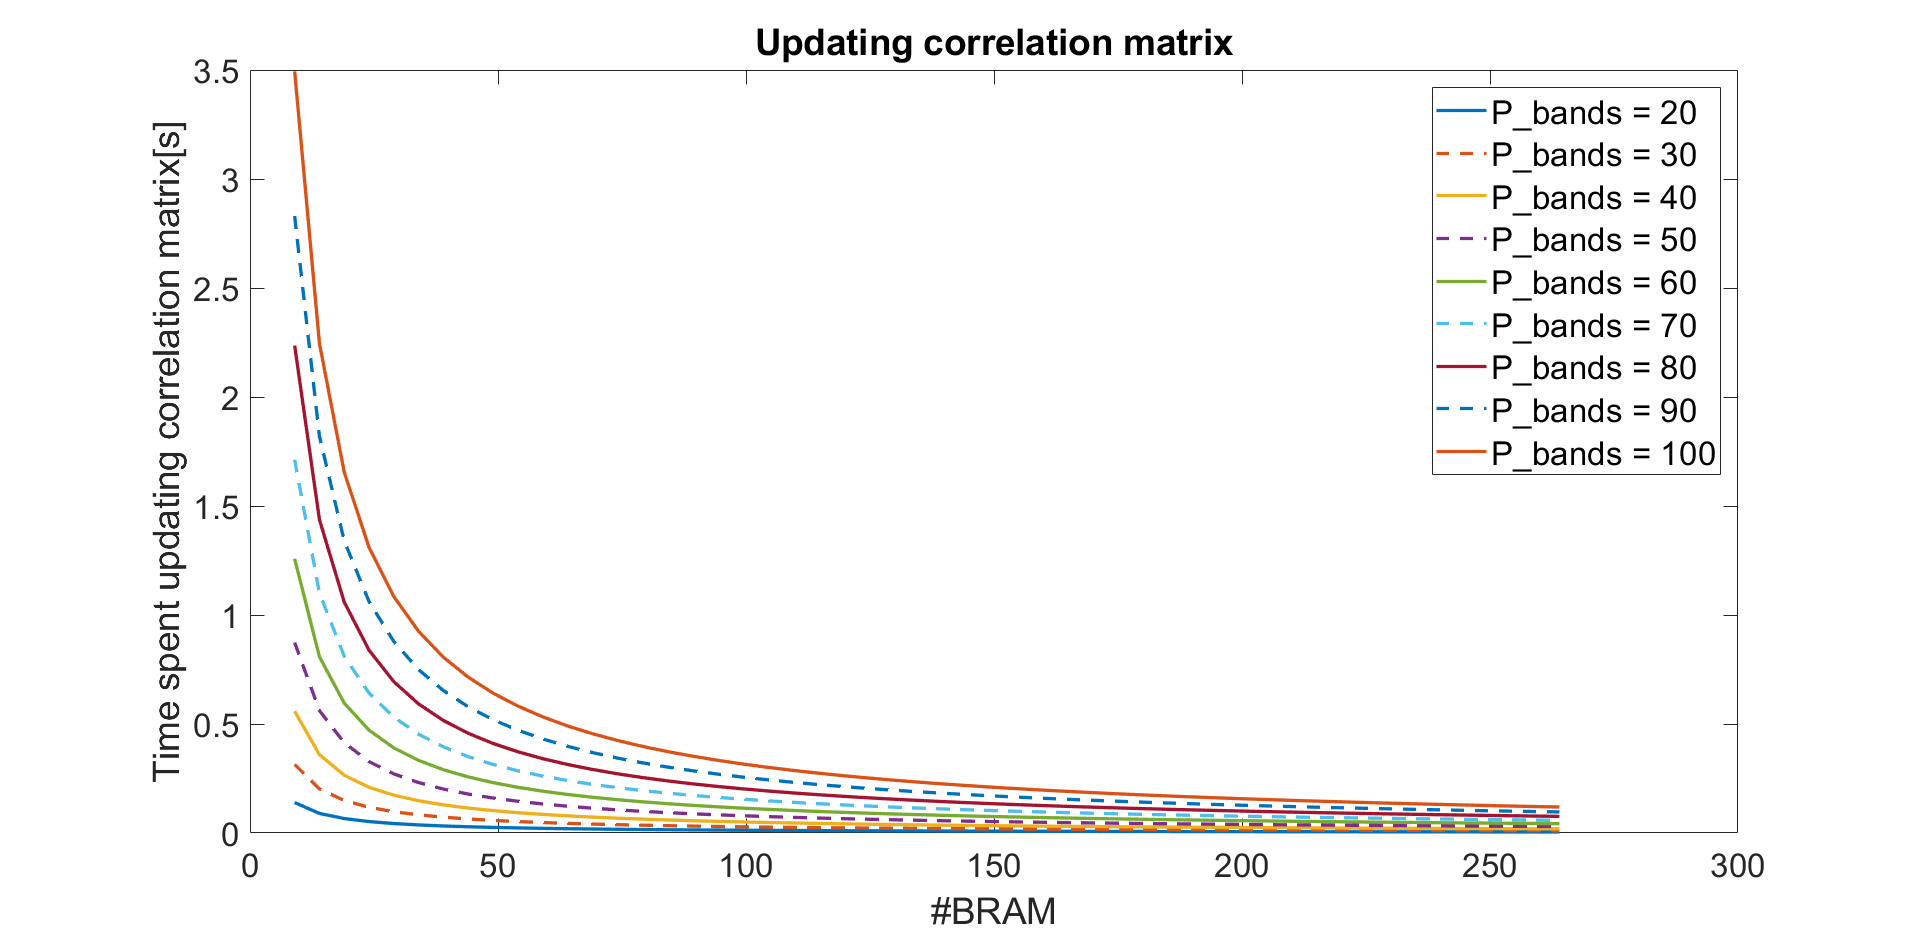
\includegraphics[scale=0.3]{images/time_spent_updating_correlation_matrix.png}}
  \caption{Estimated time spent updating $\Tilde{\textbf{R}}(\textbf{x}_k)$. } 
  \label{fig:update_time_correlation_BRAM}
\end{figure}

As shown in Figure \ref{fig:update_time_correlation_BRAM} the time spent updating $\Tilde{\textbf{R}}(\textbf{x}_k)$ can be reduced by increasing number of 36kbit BRAMs used to store the matrix. One column of $\Tilde{\textbf{R}}(\textbf{x}_k)$ will maximum contain 100 $\times$ 32=3200 bit of data. By setting $N\_bram\_correlation$ = $P\_bands$ it is possible to store one column of the correlation matrix in each BRAM, and enable writing of $P\_bands$ number of columns at the same time. As it is possible to write two 32 bit elements per cycle for each 36 kbit BRAM block, the total correlation matrix update time per pixel is $\frac{P\_bands}{2}$. 
 Storing one column in each 36 kbit BRAM block simplifies the control logic while achieving an acceptable trade off between speedup as a function of number of BRAMs used and resources used. 
 \\
 
 As the Zynq-Z7030 and the Zynq-Z7035 contains 265 and 500 BRAM blocks respectively. By utilizing $P\_bands$ to store each of the matrices in ACAD, this means maximum number of spectral bands will be [53, 100] for the Z7030 and the Z7035. %Figure \ref{fig:data_flow_cube_dma_to_inverse} shows the data flow from the Cube DMA through the ACAD correlation module, with $N\_BRAM\_correlation$ =$P\_BANDS$. 
\\



The Gauss-Jordan elimination needs to write a maximum of two rows per clock cycle to $A$ in order for each of the inner for-loops in Figure \ref{fig:gauss_jordan_pseudocode} to be executed within one clock cycle. This is needed when the operations shown in Figure \ref{fig:max_memory_requirements_gauss_jordan} are executed:

\begin{figure}[H]
\centering
%\hbox{\hspace*{-1.1cm}             
   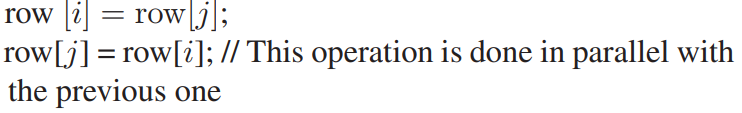
\includegraphics[scale=0.6]{images/max_memory_operations_gauss_jordan.png}%}
  \caption{Maximum memory accessing requirement by the Gauss-Jordan elimination. } 
  \label{fig:max_memory_requirements_gauss_jordan}
\end{figure}

By choosing to have $P\_bands$ number of 36 kbit BRAMs for storage of $A$ and $A^{-1}$ it is possible to write and read two rows of each matrix per clock cycle, and thereby execute the operations shown in Figure \ref{fig:max_memory_requirements_gauss_jordan} in one clock cycle. 

\\
 $\Tilde{\textbf{R}}(\textbf{x}_k)$ is written to $N\_bram\_correlation$ in parallel, where the lefter-most column (column zero) of  $\Tilde{\textbf{R}}(\textbf{x}_k)$ is written to BRAM\_0, column one to BRAM\_1,.. column P\_bands-1 to BRAM\_P\_bands-1. For each 36 kbit BRAM, two 18kbit BRAM blocks are accessed, one for even row indices of the column, and one for odd row indices of the column. In Figure \ref{fig:BRAM_matrix} the addressing scheme for each 36kbit BRAM is presented, exemplified by BRAM\_0 and BRAM\_P\_bands-1. As shown in the figure, elements of column zero is stored in BRAM\_0, while elements of column P\_BANDS-1 is stored in BRAM\_P\_bands-1.


\begin{figure}[H]
\centering
\hbox{\hspace*{-1cm}             

   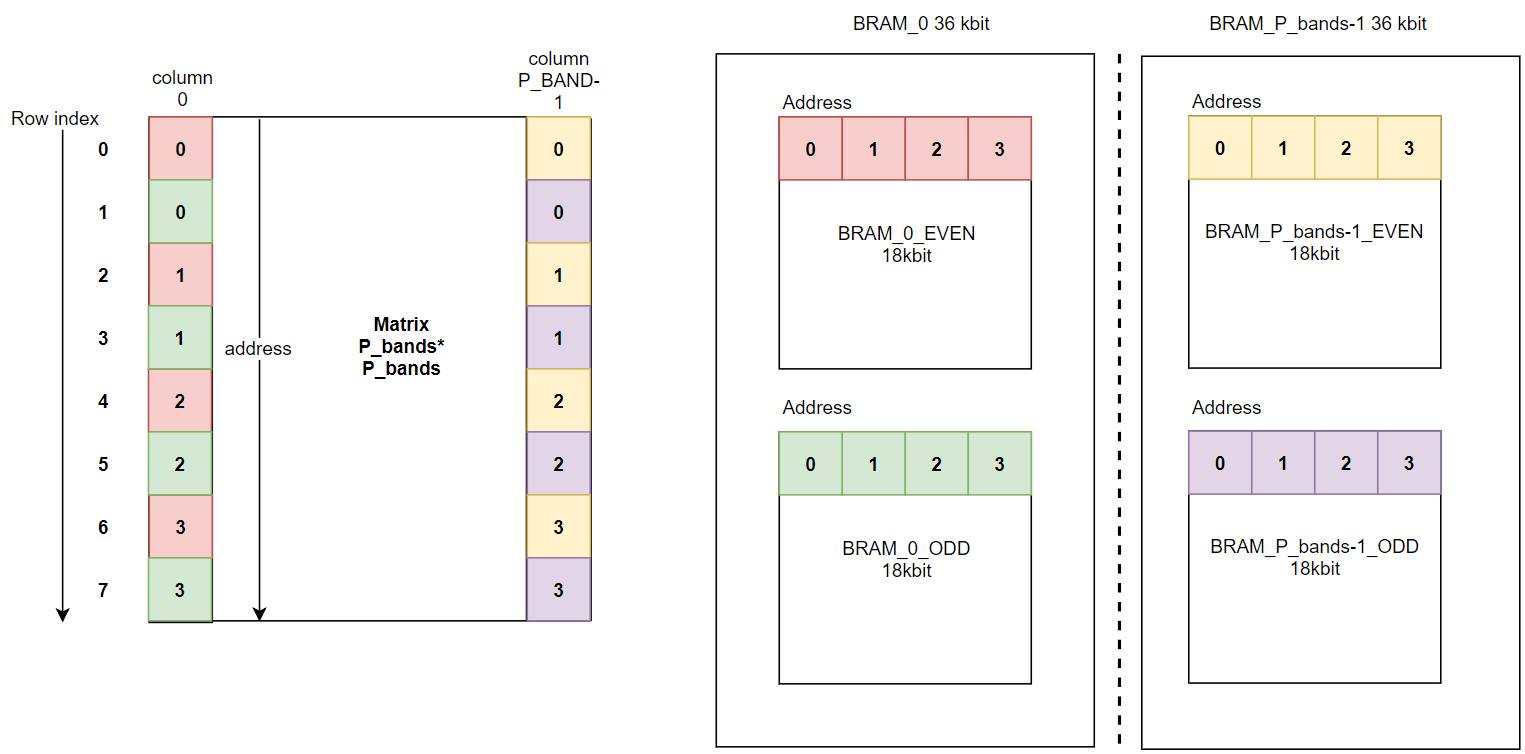
\includegraphics[scale=0.35]{images/bram_addressing_matrix.PNG}}
  \caption{Addressing scheme for storage of matrices utilized by ACAD in BRAM. One column of the matrix is stored per 36kbit BRAM.} 
  \label{fig:BRAM_matrix}
\end{figure}

 By using the same addressing logic for $\textbf{R(x}_k)$, $\sum_{t_j\in\Delta(k)}\textbf{t}_j\textbf{t}_j^T$,  $A$ and $A^{-1}$  as for $\Tilde{\textbf{R}}(\textbf{x}_k)$, the control logic of the design is simplified. \\



Figure \ref{fig:BRAM_hierarchy} shows a 36 kbit BRAM block used in the design and the dataflow within.

\begin{figure}[H]
\centering

   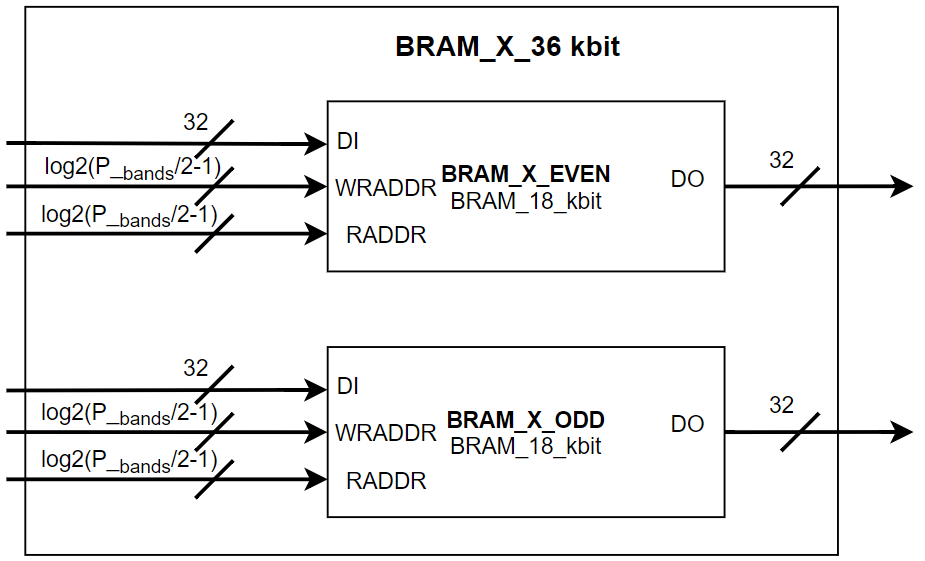
\includegraphics[scale=0.5]{images/BRAM_two_18_kbit.PNG}
  \caption{BRAM hierarchy, showing two 18kbit BRAM blocks contained within one 36kbit BRAM block. } 
  \label{fig:BRAM_hierarchy}
\end{figure}

\textbf{BRAM\_X\_EVEN} contains even row index elements for column X. \textbf{BRAM\_X\_ODD} contains odd row indexes of the column for the same column. The width of the addresses $WRADDR$ and $RADDR$ will be $log_2(\frac{P\_bands}{2})$. This is because a maximum of $\frac{P\_bands}{2}$ addresses is needed as one 36kbit BRAM contains two 18kbit BRAM blocks, storing even and odd indexes of the column, as shown in Figure \ref{fig:BRAM_matrix}. This means half the column is stored in the \textbf{BRAM\_X\_EVEN}, and the other half in the \textbf{BRAM\_X\_ODD}. 







\section{Proposed implementation}

The top level architecture of the ACAD Anomaly detector is shown in Figure \ref{fig:top_level_ACAD}. It consists of five blocks; \textbf{FSM ACAD}, \textbf{Shiftregister}, \textbf{ACAD correlation}, \textbf{ACAD inverse} and \textbf{dACAD module}. The matrices $\textbf{R(x}_k)$, $\sum_{t_j\in\Delta(k)}\textbf{t}_j\textbf{t}_j^T$,  $A$ , $A^{-1}$ and $\Tilde{\textbf{R}}(\textbf{x}_k)$ are all stored in BRAM. The ACAD anomaly detector interfaces the Cube DMA via an AXI-LITE interface. The output of the ACAD anomaly detector is a binary anomaly map. 

\begin{figure}[H]
\refstepcounter{figure}
\begin{tabular}{c|c}

   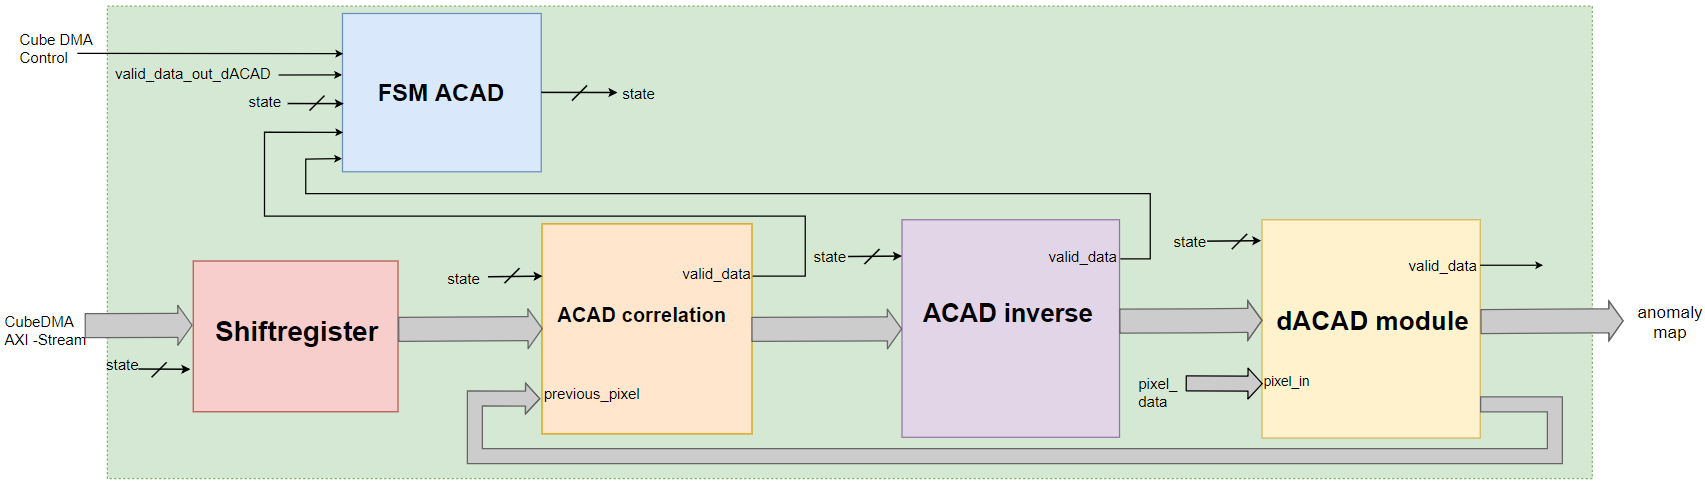
\includegraphics[scale=0.47, angle=90, origin=c]{images/acad_top_level.PNG}
   \rotatebox[origin=c]{90}{ Figure~\thefigure: Top level architecture of the ACAD anomaly detector.}
  %\caption{ \textbf{ROTATE}FSM controlling the architecture shown in Figure  } 
  \end{tabular}
  \label{fig:top_level_ACAD}
\end{figure}

The $\textbf{Shiftregister}$ is a $P\_bands$ $\times$ $Pixel\_data\_width$ $\times$ 2 wide AXI-LITE compatible shiftregister. It gets input pixel data from the CubeDMA used by the Smallsat project. 64-bit data is shifted in per clock cycle. For $Pixel\_data\_width$ of 16, four bands are shifted in per cycle. When a complete pixel is shifted in, it is sent to the $\textbf{ACAD correlation}$, which computes the matrix $\Tilde{\textbf{R}}(\textbf{x}_k)$. After $\Tilde{\textbf{R}}(\textbf{x}_k)$ is computed, it is sent to $\textbf{ACAD inverse}$. Two rows of $\Tilde{\textbf{R}}(\textbf{x}_k)$ is outputted per clock cycle to $\textbf{ACAD inverse}$, which computes $\Tilde{\textbf{R}}^{-1}(\textbf{x}_k)$.\\

Two rows of $\Tilde{\textbf{R}}^{-1}(\textbf{x}_k)$ is then sent to the $\textbf{dACAD module}$ per clock cycle. This block computes $\delta^{ACAD}$, as shown in Equation \ref{eq:ACAD_2}: 


\begin{equation}
    \delta^{ACAD}(\textbf{x}_k)= \textbf{x}_k^T\Tilde{\textbf{R}}^{-1}(\textbf{x}_k)\textbf{x}_k.
    \label{eq:ACAD_2}
\end{equation}

$u_k$ and $t_k$ is calculated in this block to decide if the pixel is anomalous or not. A binary anomaly map is created. When all pixels have been processed, the generated anomaly map is outputted, and the ACAD anomaly detection is finished.   
\\

The $\textbf{FSM\_ACAD}$ block controls the state of the ACAD anomaly detector. It chooses which of the blocks should have its clock enabled, and controls the general behaviour of the anomaly detector. 


%\section{Memory considerations}
%%\label{sec:memory_management}
 %   As the ACAD anomaly detector is to be implemented on a Zynq Z-7030 or Z-7035 device, care must be taken when designing, with respect to logic and memory usage. As the hyperspectral image data inputted to the AD might have $P\_BANDS$=100, with 16-bit image data per spectral band, memory usage is an important consideration.   





\section{Shiftregister}
The \textbf{Shiftregister} interfaces the SmallSats Cube direct memory access (DMA). The Cube DMA has a AXI-LITE interface, with a data field with a maximum size of 64 bit. Four spectral bands of a pixel vector is assumed shifted in per clock cycle. \textbf{Shiftregister} is designed to function for $P\_bands$ dividable by four, i.e. the remainder of $\frac{P\_bands}{4}$ is zero. 
%For $Pixel\_data\_width$ of 16, four bands of a pixel vector \textbf{x} are shifted in per clock cycle. 
Figure \ref{fig:shiftregister_architecture} shows the architecture of the \textbf{Shiftregister}. Figure \ref{fig:shiftregister_data_out} shows the output of the shiftregister. 

\begin{figure}[H]
\centering
\hbox{\hspace*{-1.2cm}             
   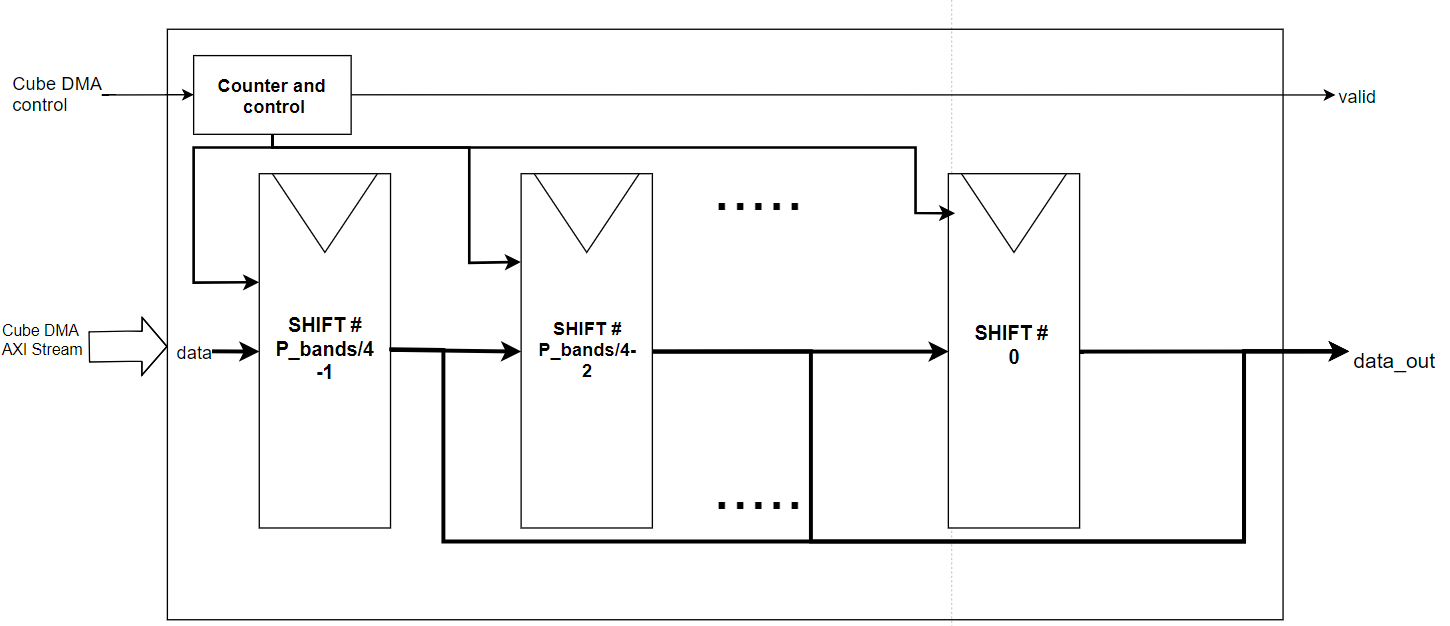
\includegraphics[scale=0.5]{images/shiftregister.png}}
  \caption{Architecture of the \textbf{Shiftregister} block. } 
  \label{fig:shiftregister_architecture}
\end{figure}


\begin{figure}[H]
\centering
   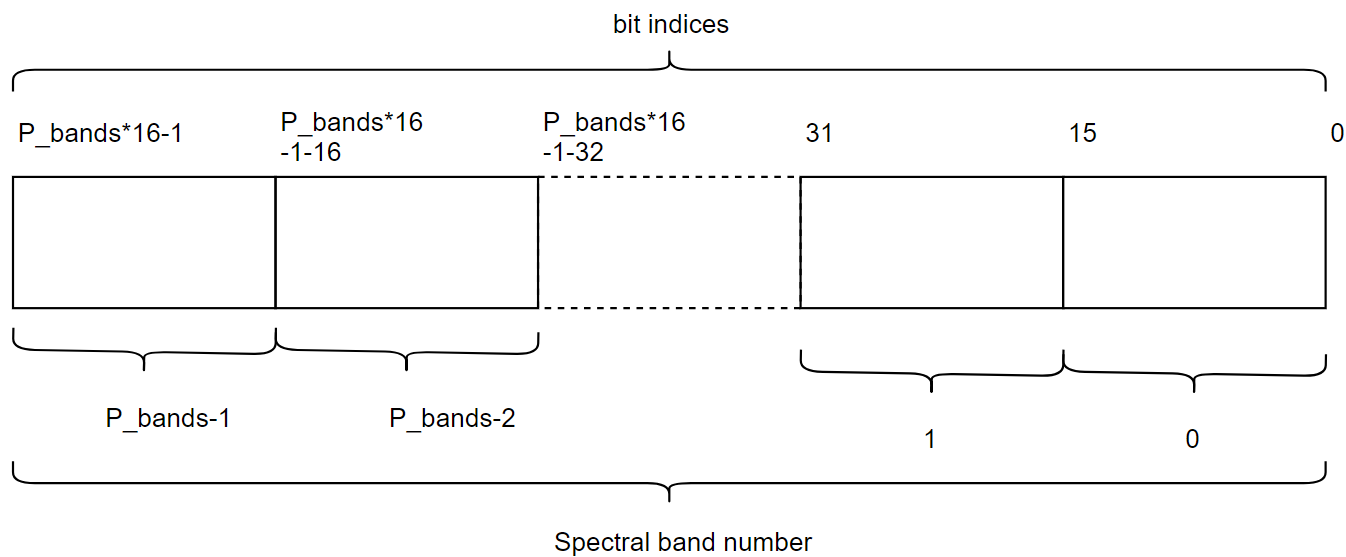
\includegraphics[scale=0.3]{images/data_format_shiftregister.PNG}
  \caption{Data output of the \textbf{Shiftregister} block. } 
  \label{fig:shiftregister_data_out}
\end{figure}



\section{ACAD correlation}
\label{sec:correlation_hw}
The \textbf{ACAD correlation}, as shown in Figure \ref{fig:top_level_ACAD}, computes the ACAD correlation matrix $\Tilde{\textbf{R}}(\textbf{x}_k)$.
\\

%As the SmallSat project is in the early phases, the value of $P\_bands$ for the data inputted to the AD from preprocessing steps are insecure. Another insecurity is the performance of the ACAD AD using PCA pre-processing, i.e. reducing the number of spectral bands in the AD. In addition, the ACAD AD requires storing of the inverse matrix, and the sum of anomaly detected. This is shown in figure X ( insert a figure showing the equation and what needs to be stored where). It is therefore not desirable to store the entire correlation matrix in flip flops, as there will be a need for storing other matrices, either in BRAM or DRAM, thereby inserting a bottleneck in the pipeline relative to the flip flop-updating step. Using BRAMs it is also possible to make a scalable solution for both small and large $p$. 
\\





%\begin{figure}[H]
%\centering
%   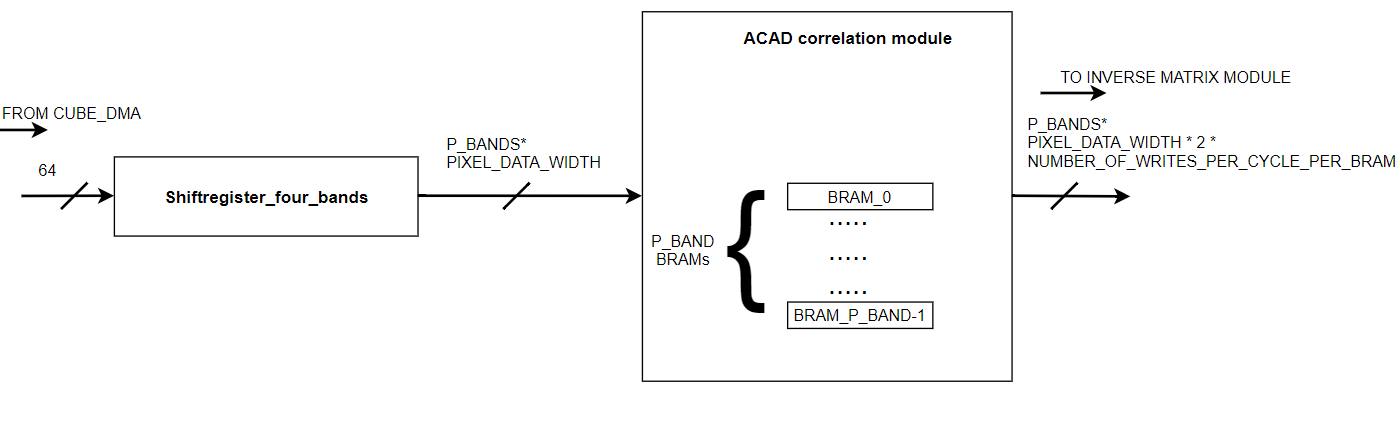
\includegraphics[scale=0.5]{images/data_flow_cube_dma_to_inverse_module.PNG}
%  \caption{Data flow from Cube DMA via shiftregister to correlation module. Output on right hand side are input for inverse matrix computation module.  } 
%  \label{fig:data_flow_cube_dma_to_inverse}
%\end{figure}

%Setting $N\_BRAMS\_correlation$ = $P\_BANDS$ allows to write to $P\_BANDS$ number of columns of the correlation matrix at the same time. 

The design is made for an even number of $P\_bands$. If odd number of spectral band is used, a band with zero values has to be inserted or the matrix needs to be re-scaled to an even number of $P\_bands$ before inputting to the \textbf{ACAD correlation}.\\


% THIS IS HIGHLY insecure
%The design is made to be scalable with $P\_bands$, and will synthesize $P\_bands$ 36 kbit BRAMs and $P\_bands$ $\times$ 2 DSP48E1 (used for multiplication).
Data flow and architecture of the correlation module can be seen in Figure \ref{fig:data_flow_correlation}. 

%NUMBER_OF_WRITES_PER_CYCLE_PER_BRAM

\begin{figure}[H]
\centering
   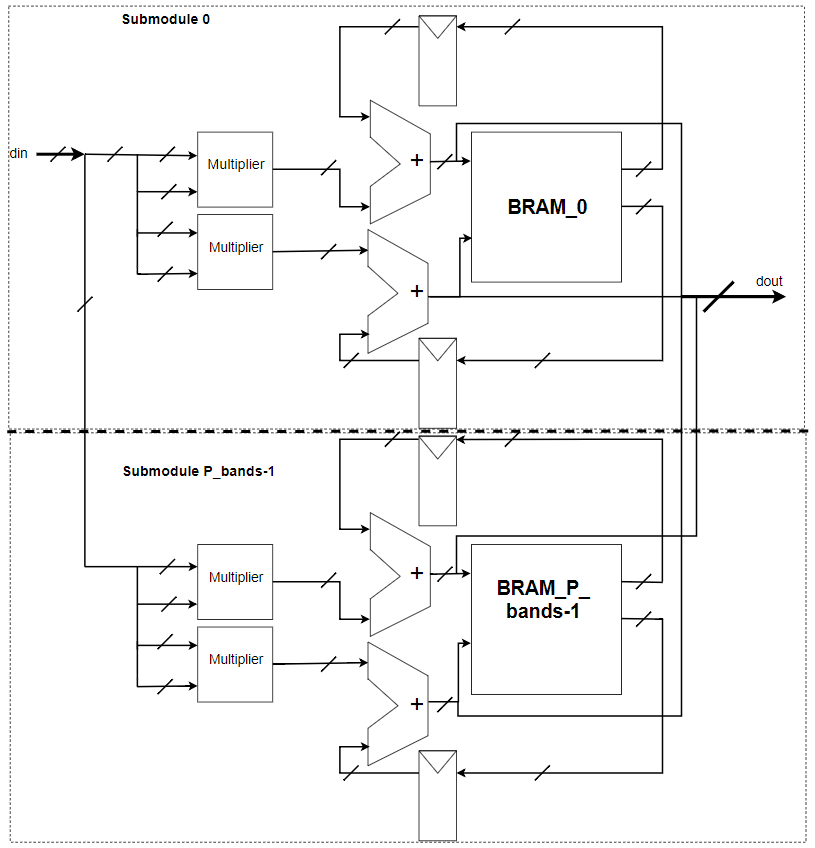
\includegraphics[scale=0.4]{images/correlation_data_path.PNG}
  \caption{Data flow within the correlation module.  } 
  \label{fig:data_flow_correlation}
\end{figure}

The dotted square marks one correlation sub-module. One correlation sub-module computes two elements of $\Tilde{\textbf{R}}(\textbf{x}_k)$.  $P\_bands$ such modules are synthesized in the design. $dout$ is a $P\_bands$ $\times$
$(Pixel\_data\_width*2)$ $\times$ 2 wide bus. $din$ is a $P\_bands$ $\times$
$Pixel\_data\_width$ wide bus.





\section{Inverse computation}
\label{sec:inverse_computation_hw}
Due to its low complexity, the Gauss-Jordan elimination was chosen for implementation of inverse computation. 

$index\_i$ and $index\_j$ corresponds to the loop indices $i$ and $j$ of the \textbf{Forward elimination} and \textbf{Backward elimination}. $row\_i$ and $row\_j$ are the rows of the matrices $A$ and $A^{-1}$ indiced by $index\_i$ and $index\_j$.

%This approach utilized $P\_BANDS$ numbers of divisions, to ensure that one row of the inverse matrix could be computed in one clock cycle. The inner loop operation of forward and backward elimination in Figure \ref{fig:gauss_jordan_pseudocode} for this approach is shown in Figure .  A scaling problem became apparent, as this approach utilized too many LUTs as functions.  This is showed in the results, section \ref{sec:synthesis:luts_and_registers_inverse}. 
%Another approach was made, \textbf{INSERT figures here}..


%%\begin{figure}[H]
%%\centering
%%   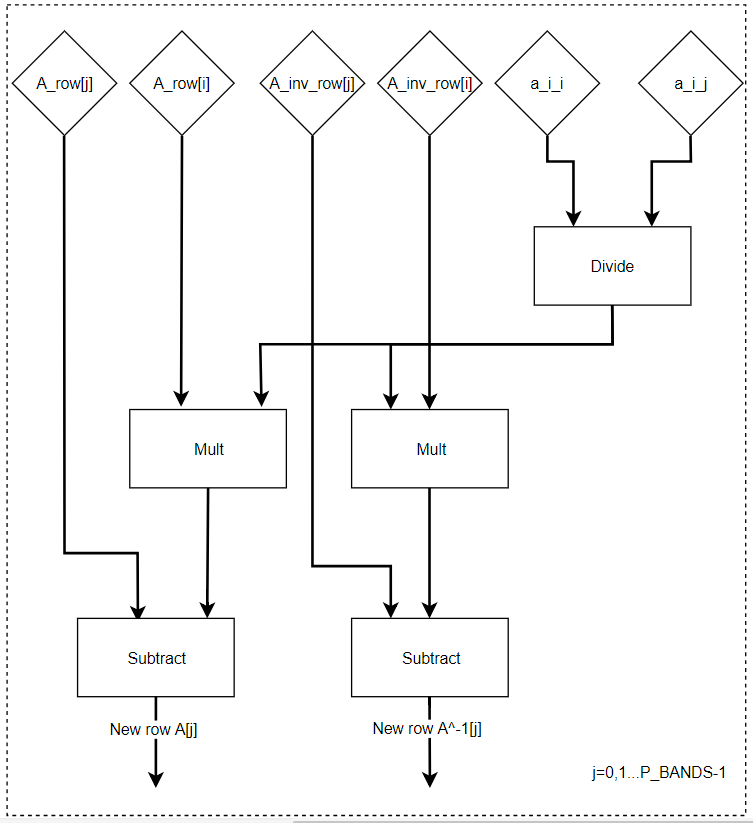
\includegraphics[scale=0.5]{images/inverse_approach_P_BANDS_divisions/inverse_core_old_approach.PNG}
%%  \caption{Architecture showing the first approach to implementing the forward and backward inner loop operation from Figure \ref{fig:gauss_jordan_pseudocode}. $P\_BANDS$ modules marked by the dotted border was synthesized.  } 
%%  \label{fig:inverse_P_BANDS_number_of_divisions}
%%\end{figure}


%\subsection{Top level architecture}
The top level architecture of \textbf{ACAD inverse} can be seen in Figure \ref{fig:top_level_inverse}. This is an implementation of the Gauss-Jordan algorithm shown in Figure \ref{fig:gauss_jordan_pseudocode}. 



\begin{figure}[H]
\refstepcounter{figure}
\begin{tabular}{c|c}

   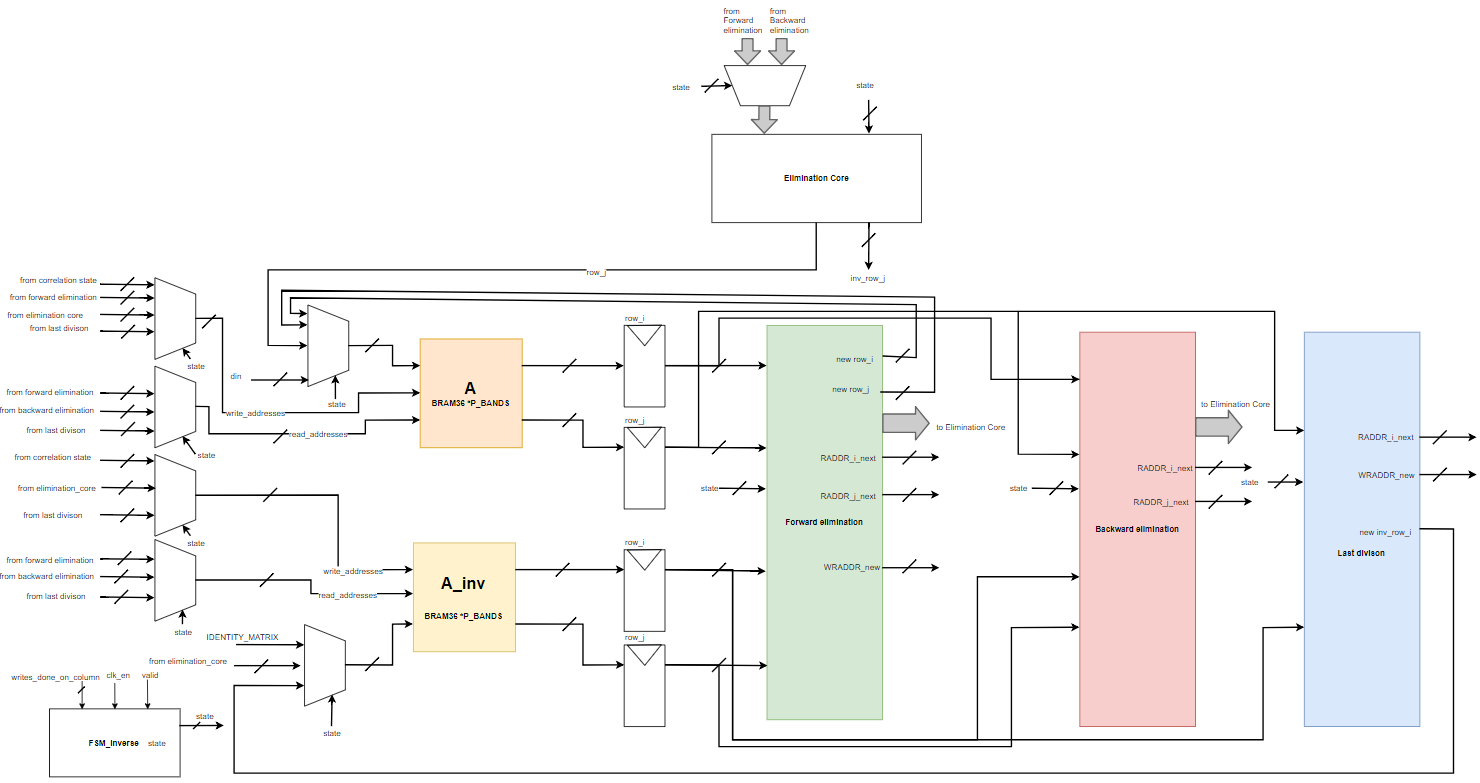
\includegraphics[scale=0.48, angle=90, origin=c]{images/inverse_hw/top_level_architecture_inverse.PNG}
   \rotatebox[origin=c]{90}{ Figure~\thefigure: Top level architecture of the inverse module.}
  %\caption{ \textbf{ROTATE}FSM controlling the architecture shown in Figure  } 
  \end{tabular}
  \label{fig:top_level_inverse}
\end{figure}


The \textbf{Forward elimination} \ref{fig:gauss_jordan_pseudocode}, \textbf{Backward elimination} and \textbf{Last division} executes the operations done in the forward elimination, backward elimination and last division part of Gauss-Jordan elimination as described in section \ref{sec:gauss_jordan_theory}, with an exception to the operations shown in Figure \ref{fig:elimination_inner_core_pseudocode}. These operations are part of both the forward elimination and backward elimination blocks in the Gauss-Jordan inverse. They are therefore put in an external process, called \textbf{Elimination core}.
$A$ and  $A\_inv$ are two arrays of BRAM36 of size $P\_bands$, in which $\textbf{A}$ and $\textbf{A}^{-1}$ are stored. 

\begin{figure}[H]
\centering
   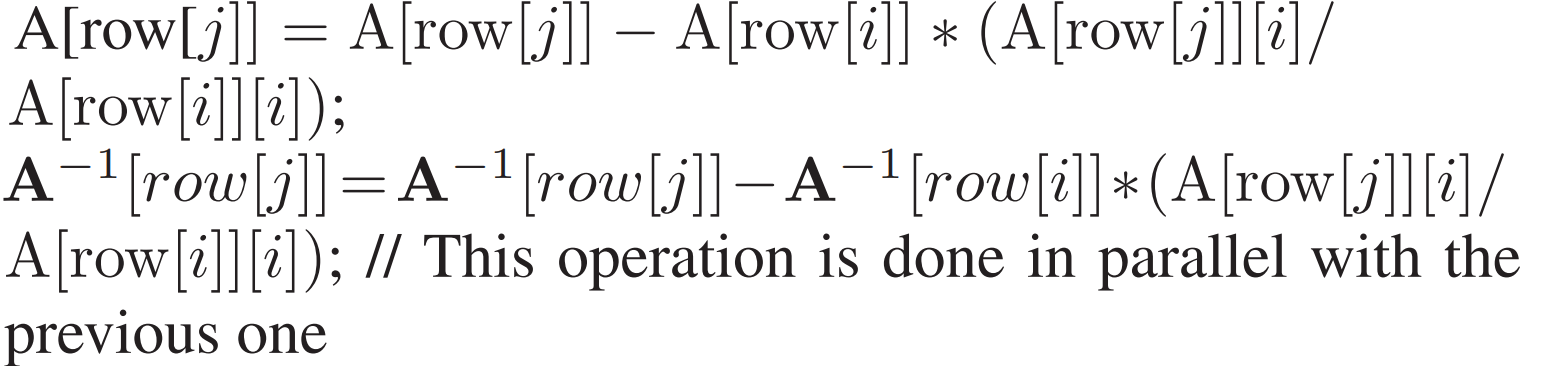
\includegraphics[scale=0.3]{images/inverse_hw/elimination_inner_core_pseudocode.PNG}
  \caption{The operations computed by the \textbf{Elimination core}, utilized by both the \textbf{Forward elimination} and the \textbf{Backward elimination} block.  } 
  \label{fig:elimination_inner_core_pseudocode}
\end{figure}



\subsection{Top level inverse FSM}
The finite state machine (FSM) for the \textbf{ACAD inverse} shown in Figure \ref{fig:top_level_inverse} is shown in Figure \ref{fig:fsm_inverse_matrix}. Its possible states are described in Table \ref{tab:fsm_inverse}.
\\

\begin{table}[H]
\centering
 \resizebox{1\textwidth}{!}
{\begin{tabular}{l|l}
State                                                                                    & Description                                                                                   \\
\hline
\textbf{Unknown state}                                                                   & An unknown state. The behaviour of the \textbf{ACAD inverse} is unknown. \\
& The FSM should transition to state \textbf{Idle}.                                    \\
\textbf{Idle}                                                                            & The \textbf{ACAD inverse} is not performing any operations.                                          \\
\textbf{\begin{tabular}[c]{@{}l@{}}Store\_correlation\_matrix\_\\ in\_BRAM\end{tabular}} & Writing data inputted from \textbf{ACAD correlation} to \textbf{A}. Two rows are \\
&written to BRAMs per clock cycle.     \\
\textbf{Forward\_elimination}                                                            & Computing the forward elimination of the Gauss-Jordan elimination.\\
\textbf{Backward\_elimination}                                                           & Computing the backward elimination of the Gauss-Jordan elimination.\\
\textbf{Last\_division}                                                                  & Computing the last division of the Gauss-Jordan elimination.              \\
\textbf{Output\_inverse\_matrix}                                                         & Outputting the completed inverse matrix for the pixel. Two rows are  \\
&outputted per clock cycle.
\end{tabular}}
\caption{States of the inverse FSM.}
\label{tab:fsm_inverse}

\end{table}

\begin{figure}[H]
\centering
   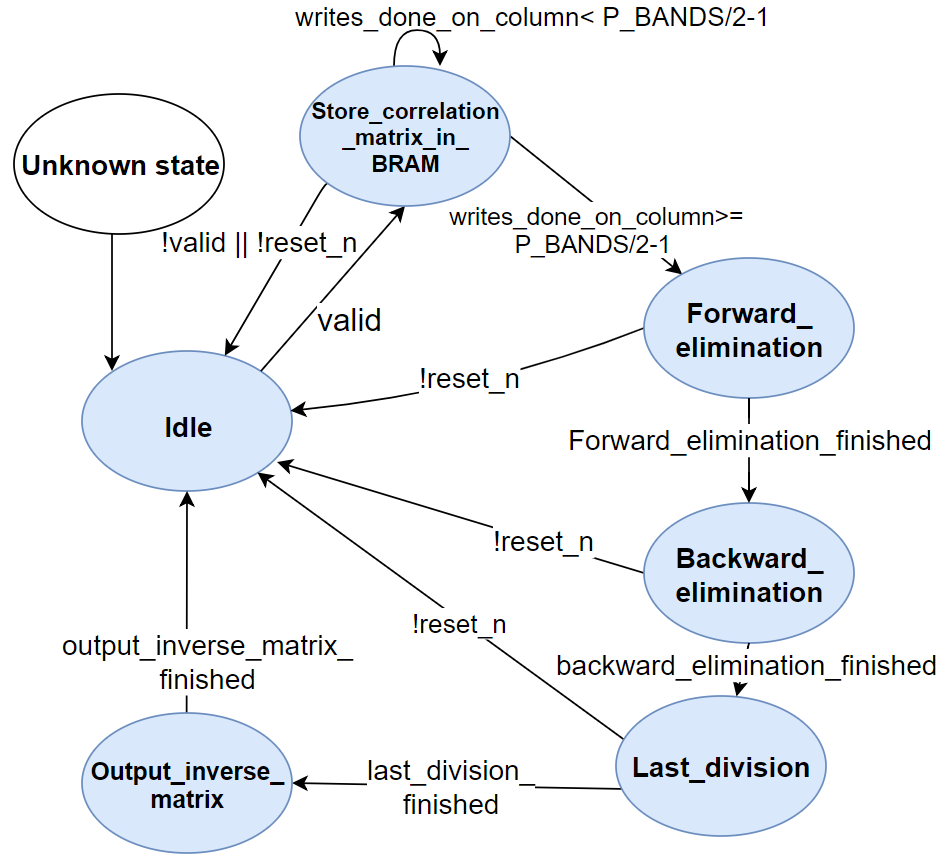
\includegraphics[scale=0.3]{images/inverse_hw/fsm_inverse_matrix.PNG}
  \caption{FSM controlling the architecture shown in Figure \ref{fig:top_level_inverse}.  } 
  \label{fig:fsm_inverse_matrix}
\end{figure}


\textbf{Idle} is a state in which \textbf{ACAD inverse} is not performing any operations. The outputs of \textbf{ACAD inverse} is not valid. \\

\textbf{Store\_correlation\_matrix\_in\_BRAM} stores two rows per clock cycle of the correlation matrix outputted from the \textbf{ACAD correlation} block in Figure \ref{fig:top_level_ACAD} in  \textbf{A} shown in Figure \ref{fig:top_level_inverse}. It also writes two rows per clock cycle of the identity matrix of size $P\_bands$ to $\textbf{A\_inv}$. \\

\textbf{Forward\_elimination} and \textbf{Backward\_elimination} computes the forward and backward elimination
of the Gauss-Jordan elimination.\\

In \textbf{Last division} the last division of the Gauss-Jordan elimination is computed.\\

\textbf{Output\_inverse\_matrix} outputs the matrix $A^{-1}$ stored in $\textbf{A\_inv}$. Two rows of the matrix is outputted per clock cycle, and sent to \textbf{dACAD}. 



\subsection{Forward elimination state}
The Forward elimination state contains a FSM with the following valid states; \textbf{Idle}, \textbf{Check\_diagonal\_element\_is\_zero}, \textbf{Swap\_rows}, \textbf{Even\_j\_write} and \textbf{Odd\_j\_write}. These are described in Table \ref{tab:fsm_forward_elimination}.

\begin{table}[H]
\centering
 \resizebox{1.\textwidth}{!}
{\begin{tabular}{l|l}
State                                                                                    & Description                                                                                   \\
\hline
\textbf{Unknown state}                                                                   & An unknown state. The behaviour of \textbf{Forward elimination} is \\ 
&unknown.The FSM should transition to state Idle.                                    \\
\textbf{Idle}                                                                            & \textbf{Forward elimination} is not performing any                                           \\
&operations.\\
\textbf{Check\_diagonal\_element\_is\_zero} & Checking if element row\_i[index\_i]= 0 as done\\ 
&in Gauss-Jordan elimination.     \\
\textbf{Swap\_rows}                                                            & Swapping $row\_i$ and $row\_j$ of  $A$ stored in \textbf{A}.        \\
\textbf{Even\_j\_write}                                                           & Updating an even indexed row of  $A$ and $A^{-1}$.       \\
\textbf{Odd\_j\_write}                                                                  & Updating an odd indexed row of  $A$ and $A^{-1}$.   
\end{tabular}}
\caption{States of the forward elimination FSM}
\label{tab:fsm_forward_elimination}

\end{table}


The FSM controlling \textbf{Forward elimination} can be seen in Figure \ref{fig:fsm_forward_elimination}.\\ $flag\_prev\_row\_i\_at\_odd\_row$ is a flag used as control to indicate whether or not the previous $row\_i$ was located at an odd indexed row. 



\begin{figure}[H]
\centering
   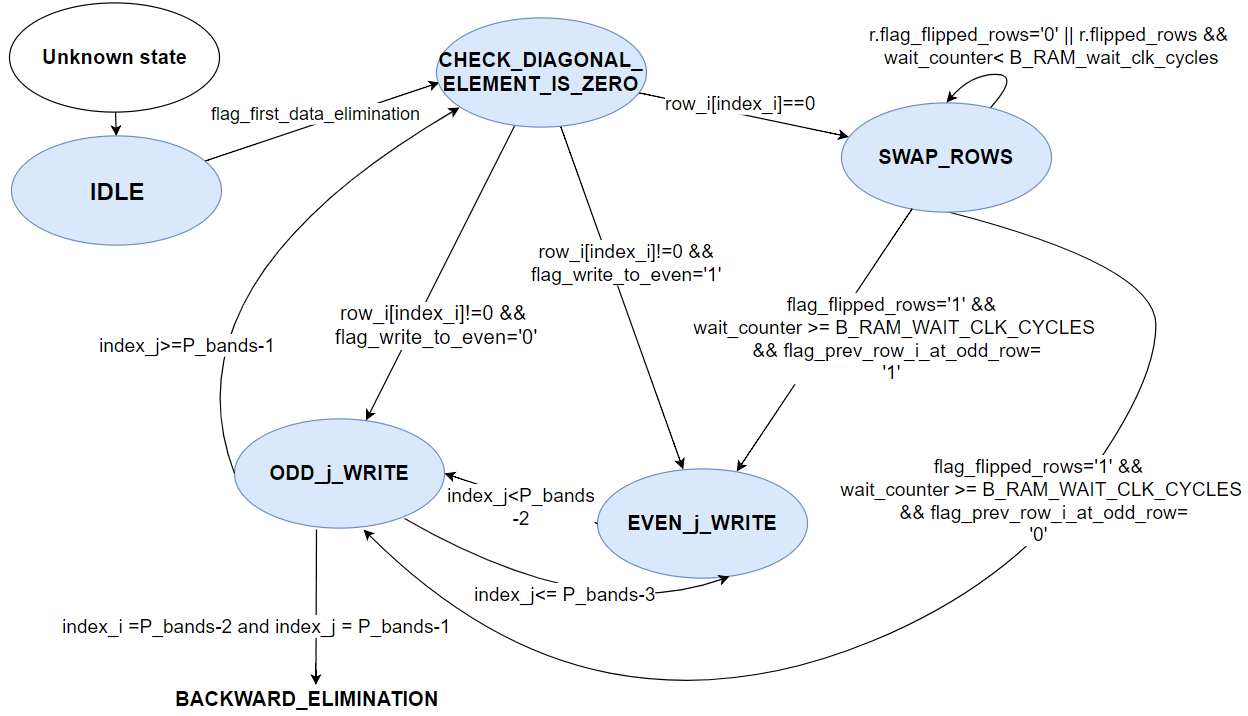
\includegraphics[scale=0.4]{images/inverse_hw/fsm_forward_elimination.png}
  \caption{FSM controlling the Forward elimination state shown in Figure \ref{fig:fsm_inverse_matrix}.  } 
  \label{fig:fsm_forward_elimination}
\end{figure}




State \textbf{Check\_diagonal\_element\_is\_zero} executes the check shown in Figure \ref{fig:check_diagonal_element}. If the check evaluates to true, the FSM transitions to state \textbf{Swap\_rows}, if it evaluates to false, it transitions to either \textbf{Even\_j\_write} or \textbf{Odd\_j\_write}, depending upon if the location of the outer loop index $i$ is at an odd or even index. 
\begin{figure}[H]
\centering
   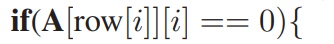
\includegraphics[scale=0.8]{images/inverse_fsms/forward_elim/check_diagonal_element_is_zero.png}
  \caption{The check done in state \textbf{Check\_diagonal\_element\_is\_zero}.  } 
  \label{fig:check_diagonal_element}
\end{figure}

\textbf{Swap rows} executes the operations shown in Figure \ref{fig:swap_rows}. When two rows are swapped the FSM needs to wait for $B\_RAM\_wait\_clk\_cycles$ before issuing transitioning to another state and issuing new reads. This is to ensure that data read is valid, and that the swap has been executed in \textbf{A}. 

\begin{figure}[H]
\centering
   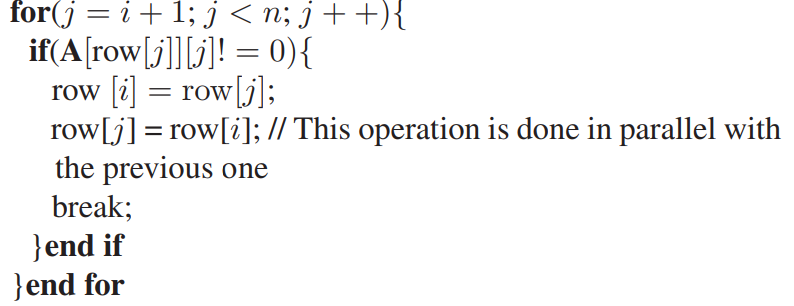
\includegraphics[scale=0.68]{images/inverse_fsms/forward_elim/swap_rows.png}
  \caption{Operations done in \textbf{Swap rows}.  } 
  \label{fig:swap_rows}
\end{figure}

\textbf{Even\_j\_write} issues writes for an even indexed row of $A$ and $A^{-1}$ to \textbf{A} and \textbf{A\_inv}. Data is structured and sent to \textbf{Elimination core}. It also issues reads to \textbf{A} and \textbf{A\_inv}. The operation of the state is illustrated in Figure \ref{fig:forward_elim_even_indexed_j}. In this example $P\_bands$ = 6, $index\_i$=0, $index\_j$=3, $w\_address$=1 and $r\_address$=2. The green row marks $row\_i$. Elements marked by red are writes being issued. Yellow elements are reads being issued. 

\begin{figure}[H]
\centering
   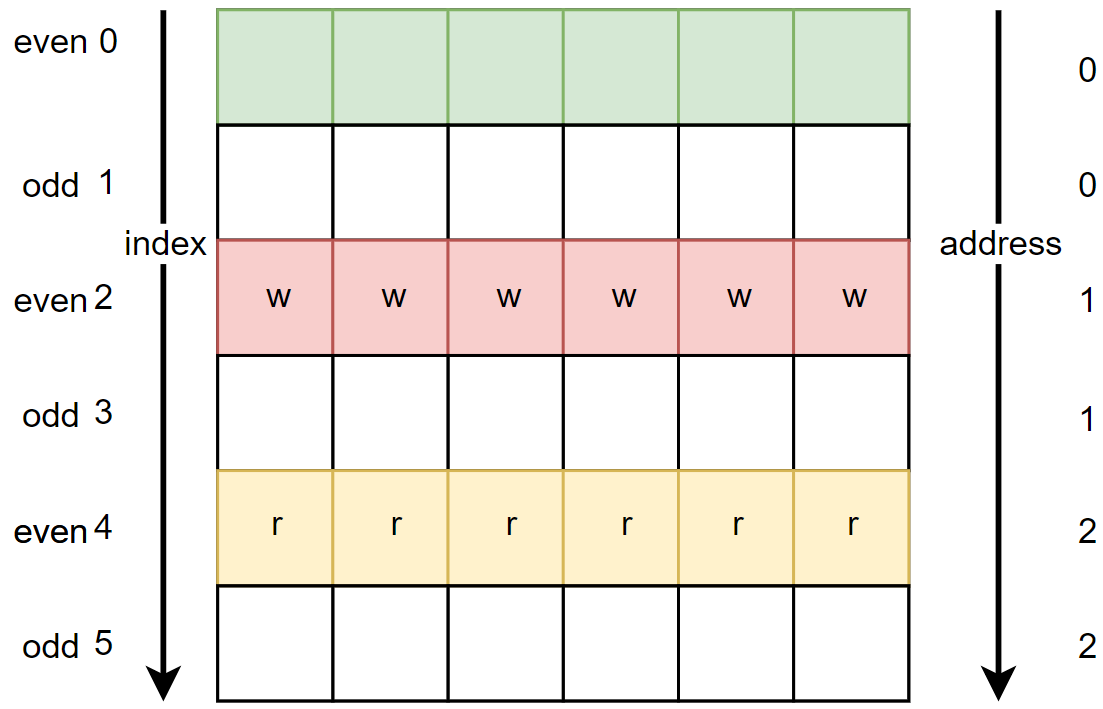
\includegraphics[scale=0.5]{images/inverse_fsms/forward_elim/write_even.PNG}
  \caption{\textbf{Even\_j\_write} in the Backward elimination state. } 
  \label{fig:forward_elim_even_indexed_j}
\end{figure}

\textbf{Odd\_j\_write} issues writes for an odd indexed row of $A$ and $A^{-1}$ to \textbf{A} and \textbf{A\_inv}. Data is structured and sent to \textbf{Elimination core}. It also issues reads to to \textbf{A} and \textbf{A\_inv}. The operation of the state is illustrated in Figure \ref{fig:forward_elim_odd_indexed_j}. In this example $P\_bands$ = 6, $index\_i$=0, $index\_j$=2, $w\_address$=1 and $r\_address$=2. 

\begin{figure}[H]
\centering
   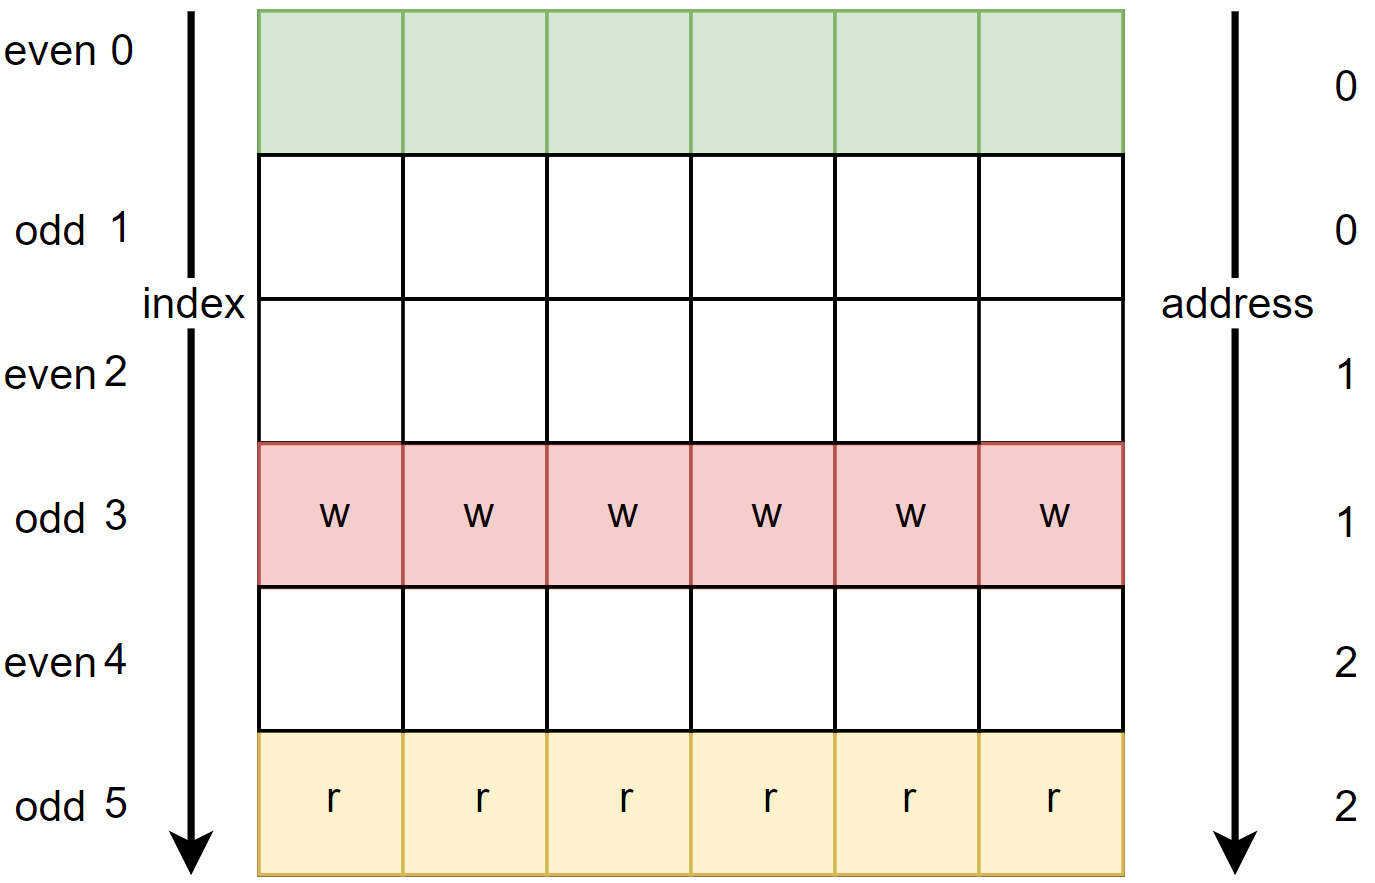
\includegraphics[scale=0.3]{images/inverse_fsms/forward_elim/write_odd.PNG}
  \caption{\textbf{Odd\_j\_write} in the forward elimination state. } 
  \label{fig:forward_elim_odd_indexed_j}
\end{figure}







%\begin{figure}[H]
%\centering
%   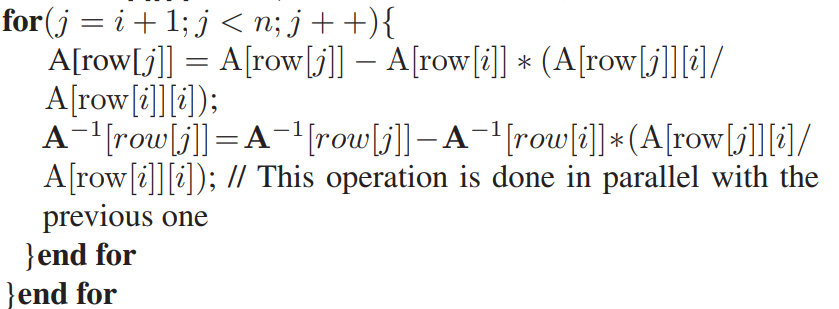
\includegraphics[scale=0.7]{images/inverse_fsms/forward_elim/even_and_odd_indexes_elimination.png}
%  \caption{Operations done \textbf{Even\_j\_write} and \textbf{Odd\_j\_write}.  } 
%  \label{fig:swap_rows}
%\end{figure}




\subsection{Backward elimination state}
The Backward elimination state contains a FSM with the following valid states; \textbf{Idle}, \textbf{First\_elimination}, \textbf{Even\_i\_start}, \textbf{Odd\_i\_start}, \textbf{Even\_j\_write} and \textbf{Odd\_j\_write}. These are shown in Table \ref{tab:fsm_backward_elimination}.


\begin{table}[H]
\centering
 \resizebox{1\textwidth}{!}
{\begin{tabular}{l|l}
State                                                                                    & Description                                                                                   \\
\hline
\textbf{Unknown state}                                                                   & An unknown state. The behaviour of the \textbf{Backward elimination} is unknown.                                     \\
&The FSM should transition to state \textbf{Idle}.\\
\textbf{Idle}                                                                            & \textbf{Backward elimination} is not performing any                                           \\
 &operations.\\
\textbf{First\_elimination} & Doing the first backward elimination iteration in the inverse    \\
& computation. The first row written will be to an even row.\\
\textbf{Odd\_i\_start}                                                            & Starting at a new iteration of the outermost loop of the backward  
\\
&elimination loop in the Gauss-Jordan elimination.\\
&
Starting at an odd row $index\_i$ of the matrix. Computing $A[row\_j]$       \\
&and $A^{-1}[row\_j]$, which is at an even index.\\

\textbf{Even\_i\_start}                                                            & Starting at a new iteration of the outermost loop of the backward 
\\
&elimination loop in the Gauss-Jordan elimination.\\
&
Starting at an even row $index\_i$ of the matrix. Computing $A[row\_j]$   \\
&and $A^{-1}[row\_j]$, which is at an odd index.\\

\textbf{Even\_j\_write}                                                           & Updating an even indexed row of $A$ and $A^{-1}$.       \\
\textbf{Odd\_j\_write}                                                                  & Updating an odd indexed row of A and $A^{-1}$.   
\end{tabular}}
\caption{States of the backward elimination FSM.}
\label{tab:fsm_backward_elimination}
\end{table}

The FSM controlling \textbf{Backward elimination} can be seen in Figure \ref{fig:fsm_inverse_matrix}.\\ $flag\_index\_i\_at\_odd\_row$ is a flag used to signal if previous $row\_i$ was located at an odd indexed row. 

\begin{figure}[H]
\centering
   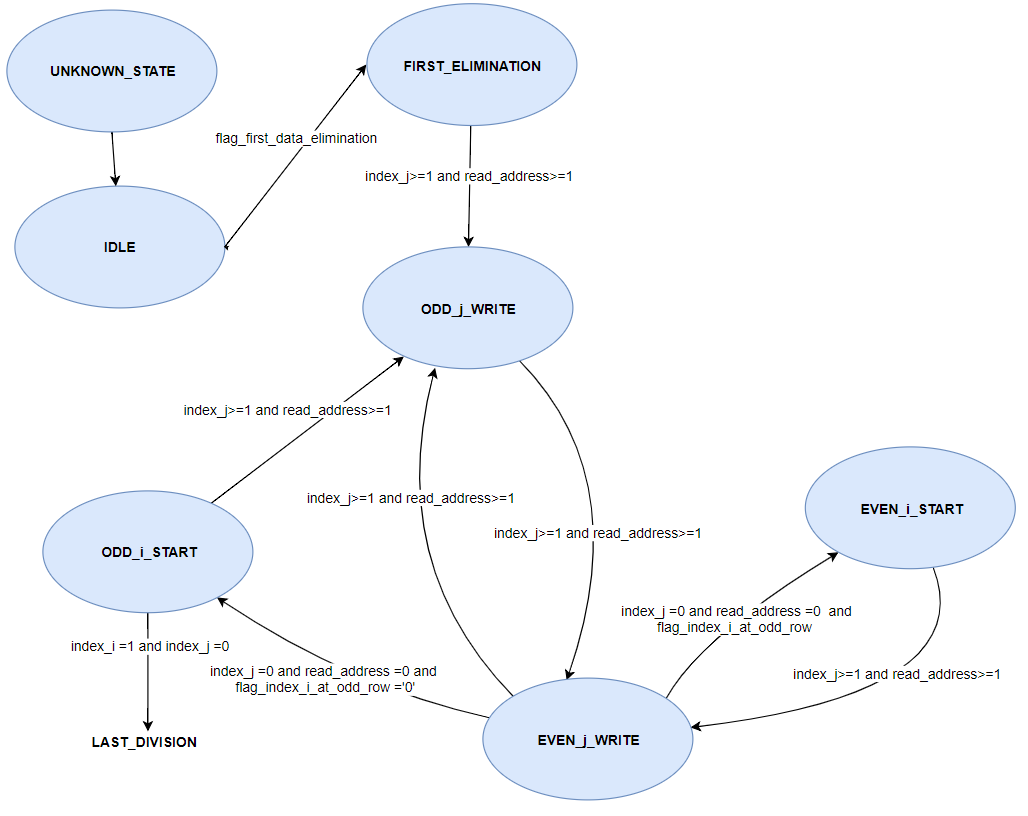
\includegraphics[scale=0.4]{images/inverse_hw/fsm_backward_elimination.PNG}
  \caption{FSM controlling the backward elimination state shown in Figure \ref{fig:fsm_inverse_matrix}.  } 
  \label{fig:fsm_backward_elimination}
\end{figure}



\textbf{First\_elimination} is the first iteration of the backward elimination. The flag $flag\_first\_data\_elimination$ is asserted once $writes\_done\_on\_column$ =$\frac{P\_bands}{2}$-1 and the two rows with index $P\_bands$-1 and $P\_bands$-2 has been read from memory. $writes\_done\_on\_column$ is a control signal outputted from \textbf{ACAD correlation}, stating the number of writes done to individual columns(BRAMs) in \textbf{A} and \textbf{A\_inv}.  \textbf{First\_elimination} will always issue a write to an even row. 

\textbf{Even\_j\_write} issues writes for an even indexed row of $A$ and $A^{-1}$ to \textbf{A} and \textbf{A\_inv}. Data is structured and sent to \textbf{Elimination core}. It also issues reads to \textbf{A} and \textbf{A\_inv}. The operation of the state is illustrated in Figure \ref{fig:backward_elim_even_indexed_j}. In this example $P\_bands$ = 6, $index\_i$=$P\_bands$-1, $index\_j$=4, $w\_address$=2 and $r\_address$=1. 

\begin{figure}[H]
\centering
   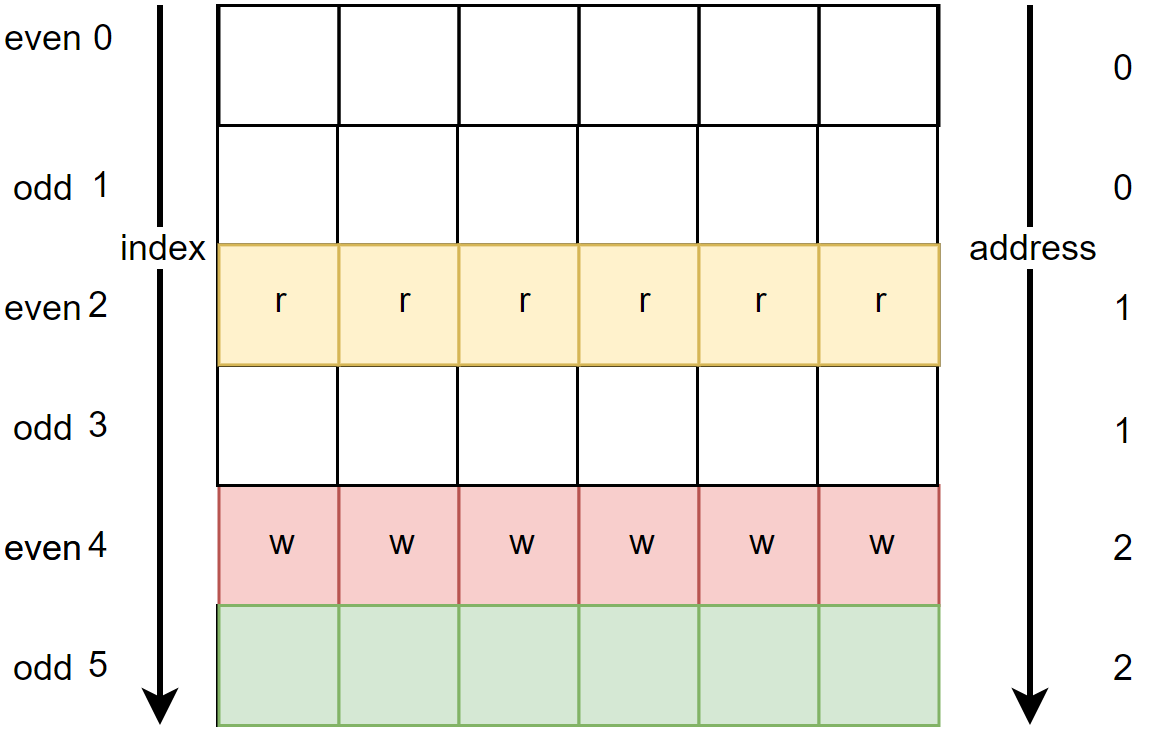
\includegraphics[scale=0.3]{images/inverse_fsms/backward_elim/write_even_j.PNG}
  \caption{\textbf{Even\_j\_write} in backward elimination. } 
  \label{fig:backward_elim_even_indexed_j}
\end{figure}

\textbf{Odd\_j\_write} issues writes for an odd indexed row of $A$ and $A^{-1}$ to \textbf{A} and \textbf{A\_inv}. Data is structured and sent to \textbf{Elimination core}. It also issues reads to \textbf{A} and \textbf{A\_inv}. The operation of the state is illustrated in Figure \ref{fig:backward_elim_odd_indexed_j}. In this example $P\_bands$ = 6, $index\_i$=$P\_bands$-1, $index\_j$=3, $w\_address$=1 and $r\_address$=0. 

\begin{figure}[H]
\centering
   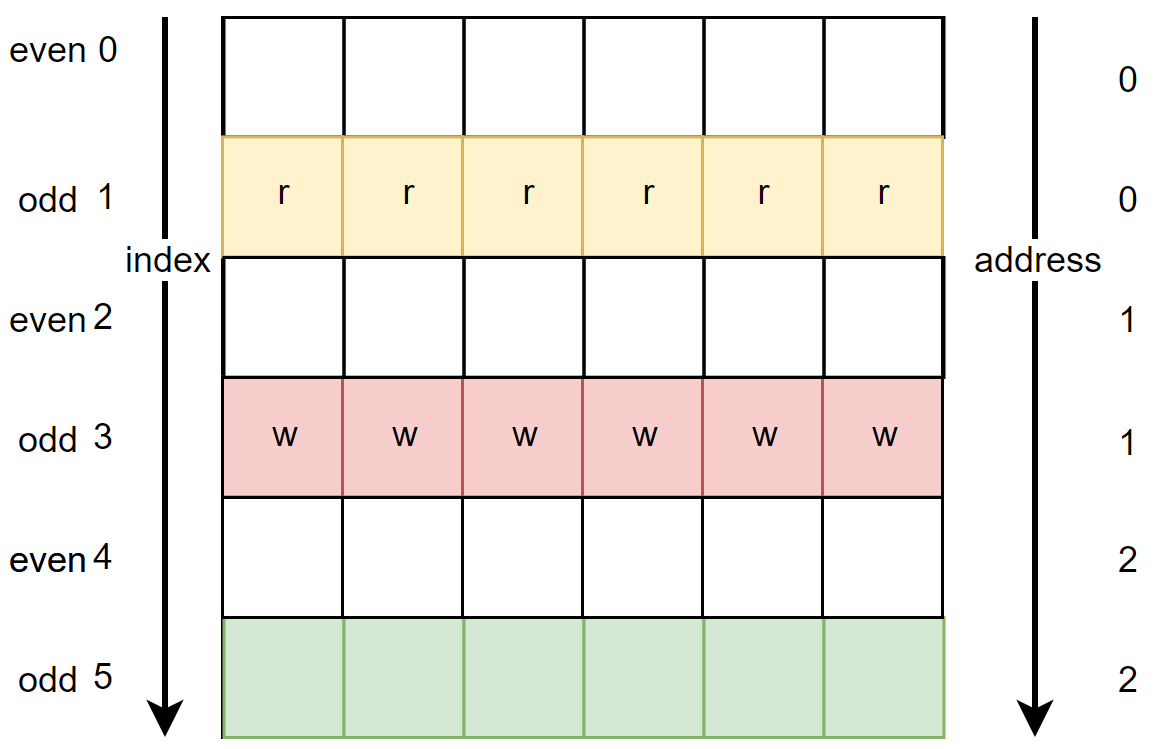
\includegraphics[scale=0.3]{images/inverse_fsms/backward_elim/write_odd_j.png}
  \caption{\textbf{Odd\_j\_write} in backward elimination. } 
  \label{fig:backward_elim_odd_indexed_j}
\end{figure}

\textbf{Odd\_i\_start} is a new iteration of the outermost loop in backward elimination. $index\_i$ is located at an odd indexed row.  In this state a write is issued to an even indexed row. An example is shown in Figure \ref{fig:odd_i_start}. In this example  $P\_bands$=6, $index\_i$=3, $index\_j$=2, $w\_address$=1 and $r\_address$=0.

\begin{figure}[H]
\centering
   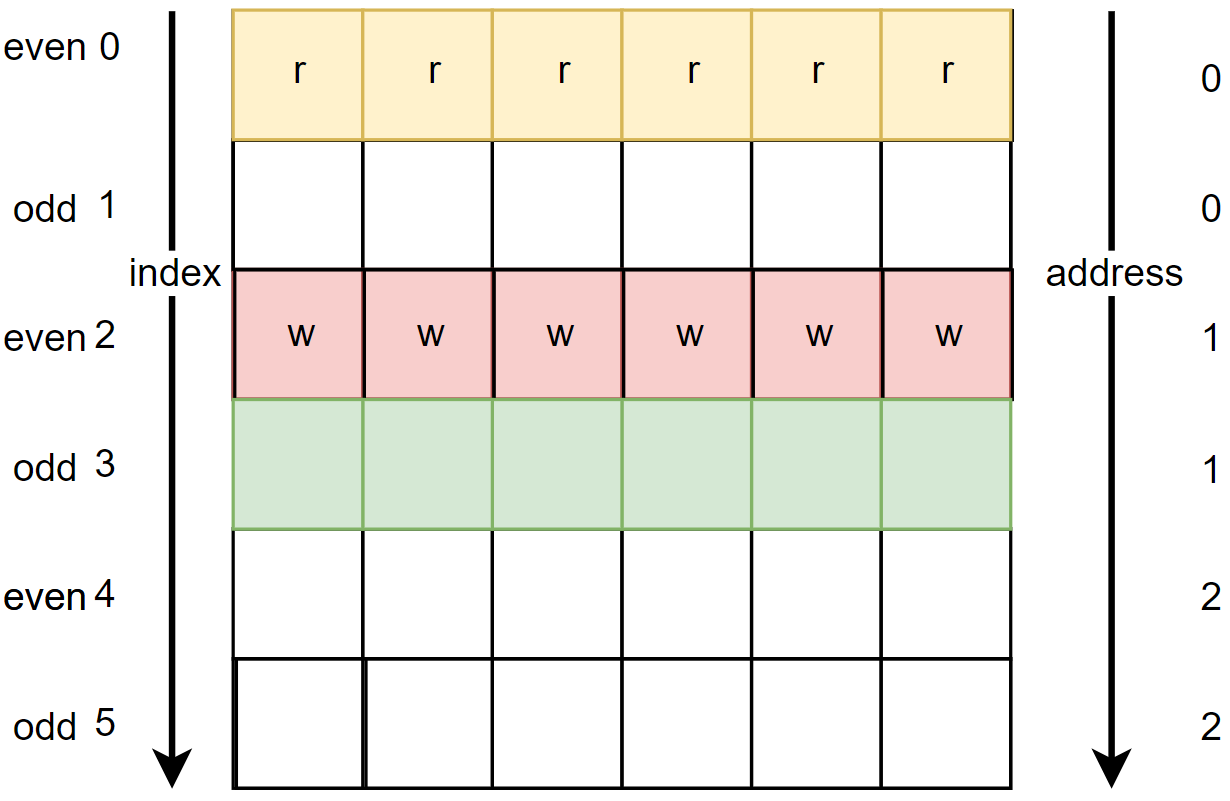
\includegraphics[scale=0.3]{images/inverse_fsms/backward_elim/odd_i_start.PNG}
  \caption{\textbf{Odd\_i\_start}. } 
  \label{fig:odd_i_start}
\end{figure}

\textbf{Even\_i\_start} is a new iteration of the outermost loop in backward elimination. $index\_i$ is located at an odd indexed row.  In this state a write is issued to an even indexed row. An example is shown in Figure \ref{fig:odd_i_start}. In this example  $P\_bands$=6, $index\_i$=4, $index\_j$=3, $w\_address$=1 and $r\_address$=0.


\begin{figure}[H]
\centering
   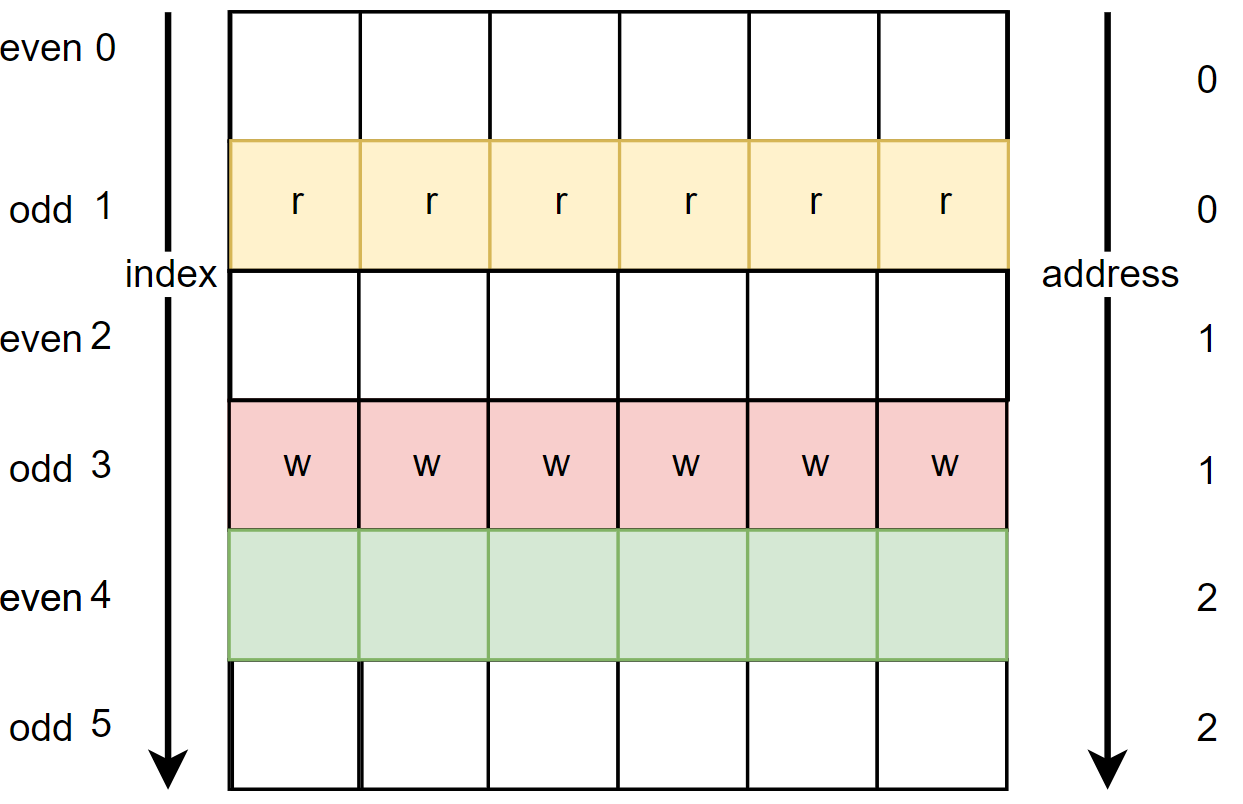
\includegraphics[scale=0.3]{images/inverse_fsms/backward_elim/even_i_start.PNG}
  \caption{\textbf{Even\_i\_start}. } 
  \label{fig:even_i_start}
\end{figure}



\subsection{Last division}
The Last division state contains a FSM with the following valid states; \textbf{Idle}, \textbf{Even\_i\_write} and \textbf{Odd\_i\_write}. These are described in Table \ref{tab:fsm_last_division}.

\begin{table}[H]
\centering
 \resizebox{1\textwidth}{!}
{\begin{tabular}{l|l}
State                                                                                    & Description                                                                                   \\
\hline
\textbf{Unknown state}                                                                   & An unknown state. The behaviour of \textbf{Last division} is unknown. \\
&The FSM should transition to state \textbf{Idle}.                                    \\
\textbf{Idle}                                                                            & \textbf{Last division} is not performing any operations.                                          \\


\textbf{Even\_i\_write}                                                           & Updating an even indexed row of $A^{-1}$.       \\
\textbf{Odd\_i\_write}                                                                  & Updating an odd indexed row of $A^{-1}$.   
\end{tabular}}
\caption{States of the last division FSM.}
\label{tab:fsm_last_division}

\end{table}

In \textbf{Even\_i\_write} an even indexed row of $A^{-1}$ is updated. A read is issued for the next even indexed row. \\

In \textbf{Odd\_i\_write} an odd indexed row of $A^{-1}$ is updated. A read is issued for the next odd indexed row. 


\begin{figure}[H]
\centering
   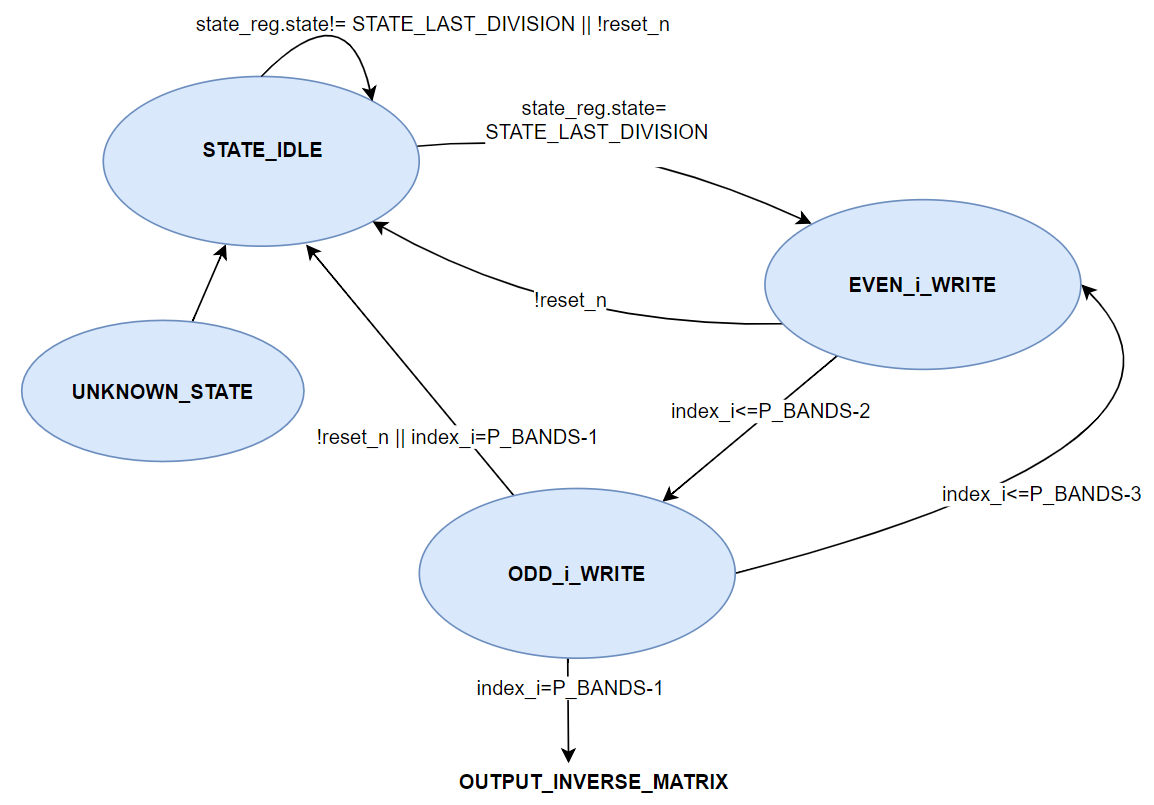
\includegraphics[scale=0.3]{images/inverse_hw/fsm_last_division.PNG}
  \caption{FSM controlling the last division state shown in Figure \ref{fig:fsm_inverse_matrix}.  } 
  \label{fig:fsm_last_division}
\end{figure}

%\subsection{Memory hierarchy}
%The Gauss Jordan inverse requires two matrices to be stored in memory, the matrix $\textbf{A}$ and $\textbf{A}^{-1}$ as shown in Figure \ref{fig:gauss_jordan_pseudocode}. Both of these matrices will be of the same size as the correlation matrix, described in section \ref{sec:mem_management_correlation_matrix}. It is therefore not desirable to store these matrices in registers, but rather in BRAM. By having the same memory structure as described in section \ref{sec:mem_management_correlation_matrix}, using $P\_BANDS$ BRAM 36kbit blocks for each of the matrices, this will enable two rows of each matrix to be written and read per clock cycle. 

\subsection{Output inverse matrix}
In the output inverse matrix state the contents of \textbf{A\_inv} is read and outputted to \textbf{dACAD}. Reading the contents off \textbf{A\_inv} takes $\frac{P\_bands}{2}$ clock cycles. 

\subsection{Inverse pipeline stages}
The inverse module is pipelined into four stages in order to achieve high throughput. The pipeline can be seen in Figure \ref{fig:pipeline_inverse_part_1}, \ref{fig:pipeline_inverse_part_2} and \ref{fig:pipeline_inverse_part_3}. The green squares mark processes in which data is written to \textbf{A}/\textbf{A\_inv}. Blue squares shows reading of data from \textbf{A}/\textbf{A\_inv}. Purple squares marks inputs being set from \textbf{FSM inverse} and \textbf{A} and \textbf{A\_inv} to \textbf{Forward elimination}, \textbf{Backward elimination}, \textbf{Elimination core} and \textbf{Last division}.  Yellow squares marks calculation of new data for $row\_j$ from the respective submodule active. 

\begin{figure}[H]
\centering
\hbox{\hspace*{-1.5cm}             

   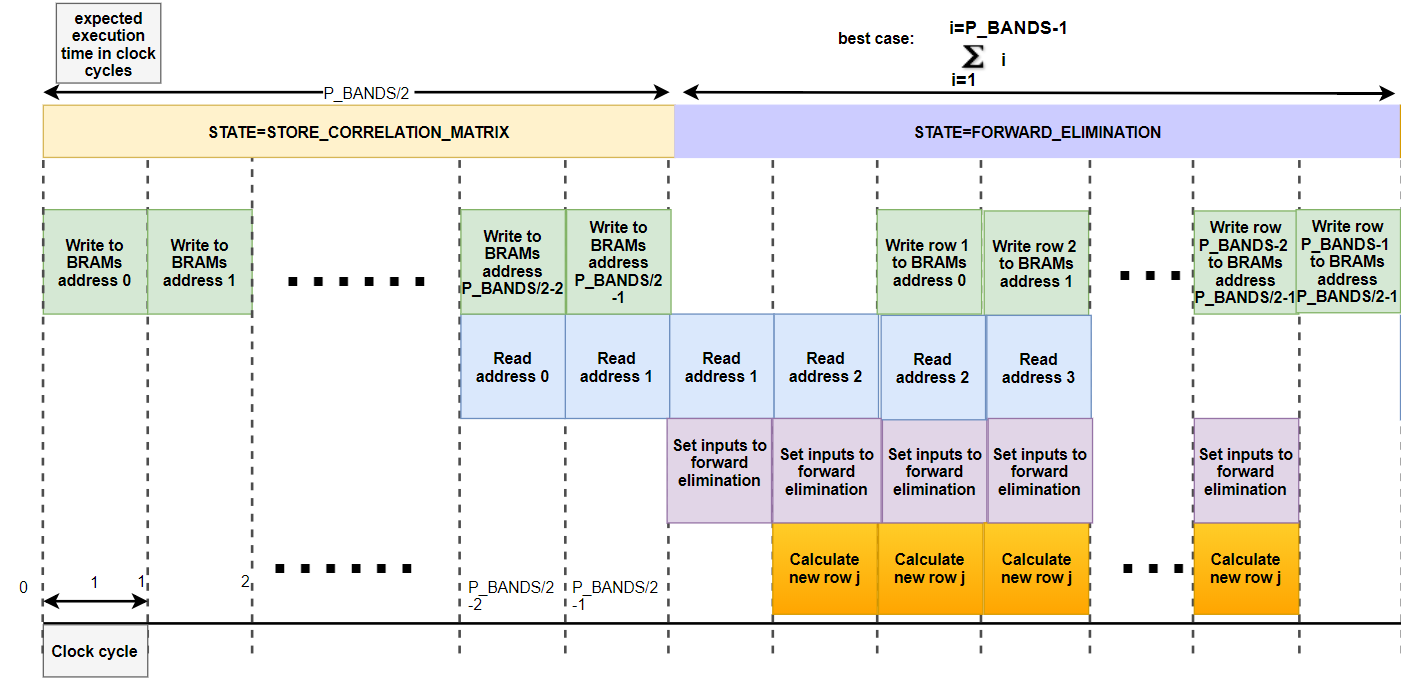
\includegraphics[scale=0.4]{images/estimation_execution_time/pipeline_inverse_matrix_part_1.PNG}}
  \caption{Showing pipeline operations in the Store\_correlation\_matrix and Forward\_elimination states.  } 
  \label{fig:pipeline_inverse_part_1}
\end{figure}

\begin{figure}[H]
\centering
\hbox{\hspace*{-1.1cm}   

   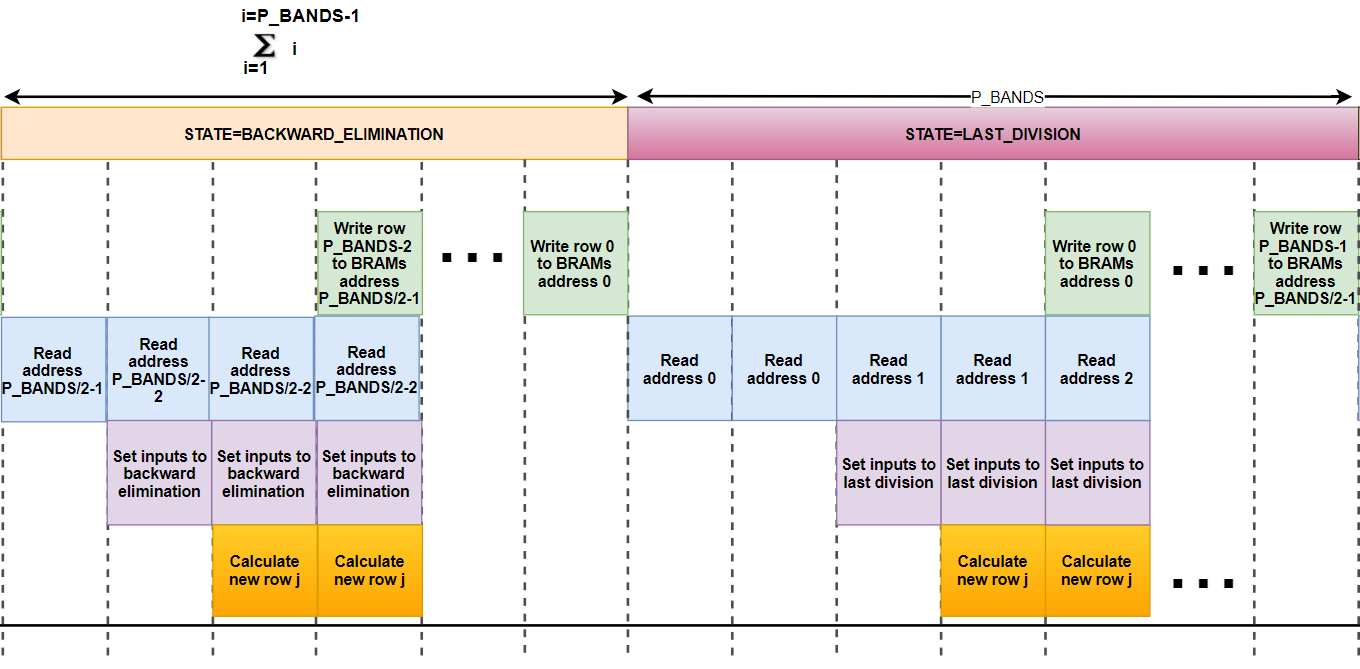
\includegraphics[scale=0.4]{images/estimation_execution_time/pipeline_inverse_matrix_part_2.PNG}}
  \caption{Showing pipeline operations in the Forward\_elimination and Last\_division states.  } 
  \label{fig:pipeline_inverse_part_2}
\end{figure}

\begin{figure}[H]
\centering

   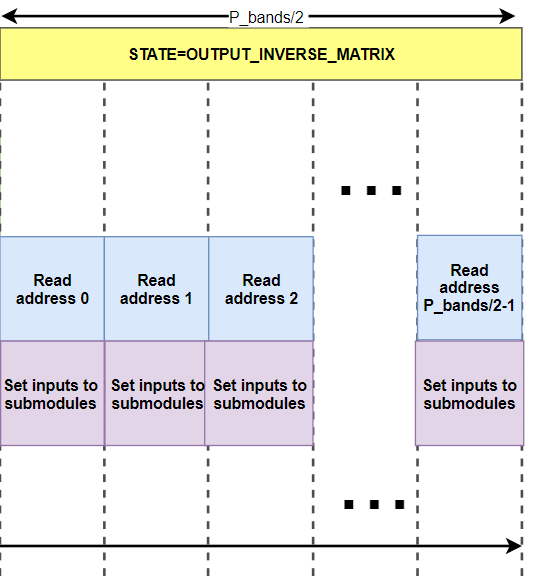
\includegraphics[scale=0.4]{images/estimation_execution_time/pipeline_inverse_matrix_part_3.PNG}
  \caption{Showing pipeline operations in the $Output\_inverse\_matrix$ state.  } 
  \label{fig:pipeline_inverse_part_3}
\end{figure}



\subsection{Execution time expectations}
Using $P\_bands$ 36 kbit BRAMs for storage of $A$ and $A^{-1}$ enables to read and write a maximum of two rows to and from \textbf{A} and \textbf{A\_inv} per clock cycle. Assuming that each of the row-operations in the Gauss-Jordan elimination can be calculated within one clock cycle, it is possible to do an estimation of the expected execution time in clock cycles for the inverse computation per pixel. \\

Expected execution time for the different states is shown in Figure \ref{fig:pipeline_inverse_part_1}, \ref{fig:pipeline_inverse_part_2} and \ref{fig:pipeline_inverse_part_3}. For state $Forward\_elimination$, the execution time will be greater if it is necessary to swap rows, done in the state \textbf{Swap rows}. The worst case execution time of $Forward\_elimination$ is assumed to be when the first element of the matrix $A$ has a zero element at row(i,i) and all other rows, except the last row, has a zero element at row(j,j). \\

A worst case and a best case execution time, $inv\_worst\_case$ and $inv\_best\_case$, for the computation of the inverse per pixel is estimated. The estimations are shown in Equation \ref{eq:inv_worst_case} and \ref{eq:inv_best_case}. $N\_STATES\_INV$ is the number of valid states in the inverse top level module, shown in Figure \ref{fig:fsm_inverse_matrix}. $worst\_case\_ex\_state$ is the set of expected worst case execution times for the states.  $best\_case\_ex\_state$ is the set of expected best case execution times for the states. 

\begin{equation}
\begin{split}
inv\_worst\_case & = \sum_{i=0}^{N\_STATES\_INV}worst\_case\_ex\_state(i) \\
& =\underbrace{\frac{P\_bands}{2} }_\text{STORE\_CORRELATION\_MATRIX}  + \overbrace{\sum_{i=0}^{P\_bands-1}i + P\_bands}^\text{STATE\_FORWARD\_ELIMINATION} \\
& + \underbrace{\sum_{i=0}^{P\_bands-1}i}_\text{STATE\_BACKWARD\_ELIMINATION}  
 +
\overbrace{P\_bands}^\text{LAST\_DIVISION} + \underbrace{P\_bands/2}_\text{OUTPUT\_INVERSE\_MATRIX}\\
& = 3P\_bands + 2\sum_{i=0}^{P\_bands-1}i
\end{split}
\label{eq:inv_worst_case}
\end{equation}


\begin{equation}
\begin{split}
inv\_best\_case & = \sum_{i=0}^{N\_STATES\_INV}best\_case\_ex\_state(i) \\
& = \underbrace{\frac{P\_bands}{2} }_\text{STORE\_CORRELATION\_MATRIX}  + \overbrace{\sum_{i=0}^{P\_bands-1}i }^\text{STATE\_FORWARD\_ELIMINATION} \\
& + \underbrace{\sum_{i=0}^{P\_bands-1}i}_\text{STATE\_BACKWARD\_ELIMINATION}  
 +
\overbrace{P\_bands}^\text{LAST\_DIVISION} + \underbrace{P\_bands/2}_\text{OUTPUT\_INVERSE\_MATRIX}\\
& = 2P\_bands + 2\sum_{i=0}^{P\_bands-1}i
\end{split}
\label{eq:inv_best_case}
\end{equation}

Figure \ref{fig:estimated_time_inverse} shows the estimated execution time in seconds for computing $\Tilde{\textbf{R}}^{-1}(\textbf{x}_k)$ for all $\textbf{x}_k$ in the hyperspectral image, for an image size of 1088x576, with a operating clock frequency of 100MHz. 

\begin{figure}[H]
\hbox{\hspace*{-2cm}                                                           

   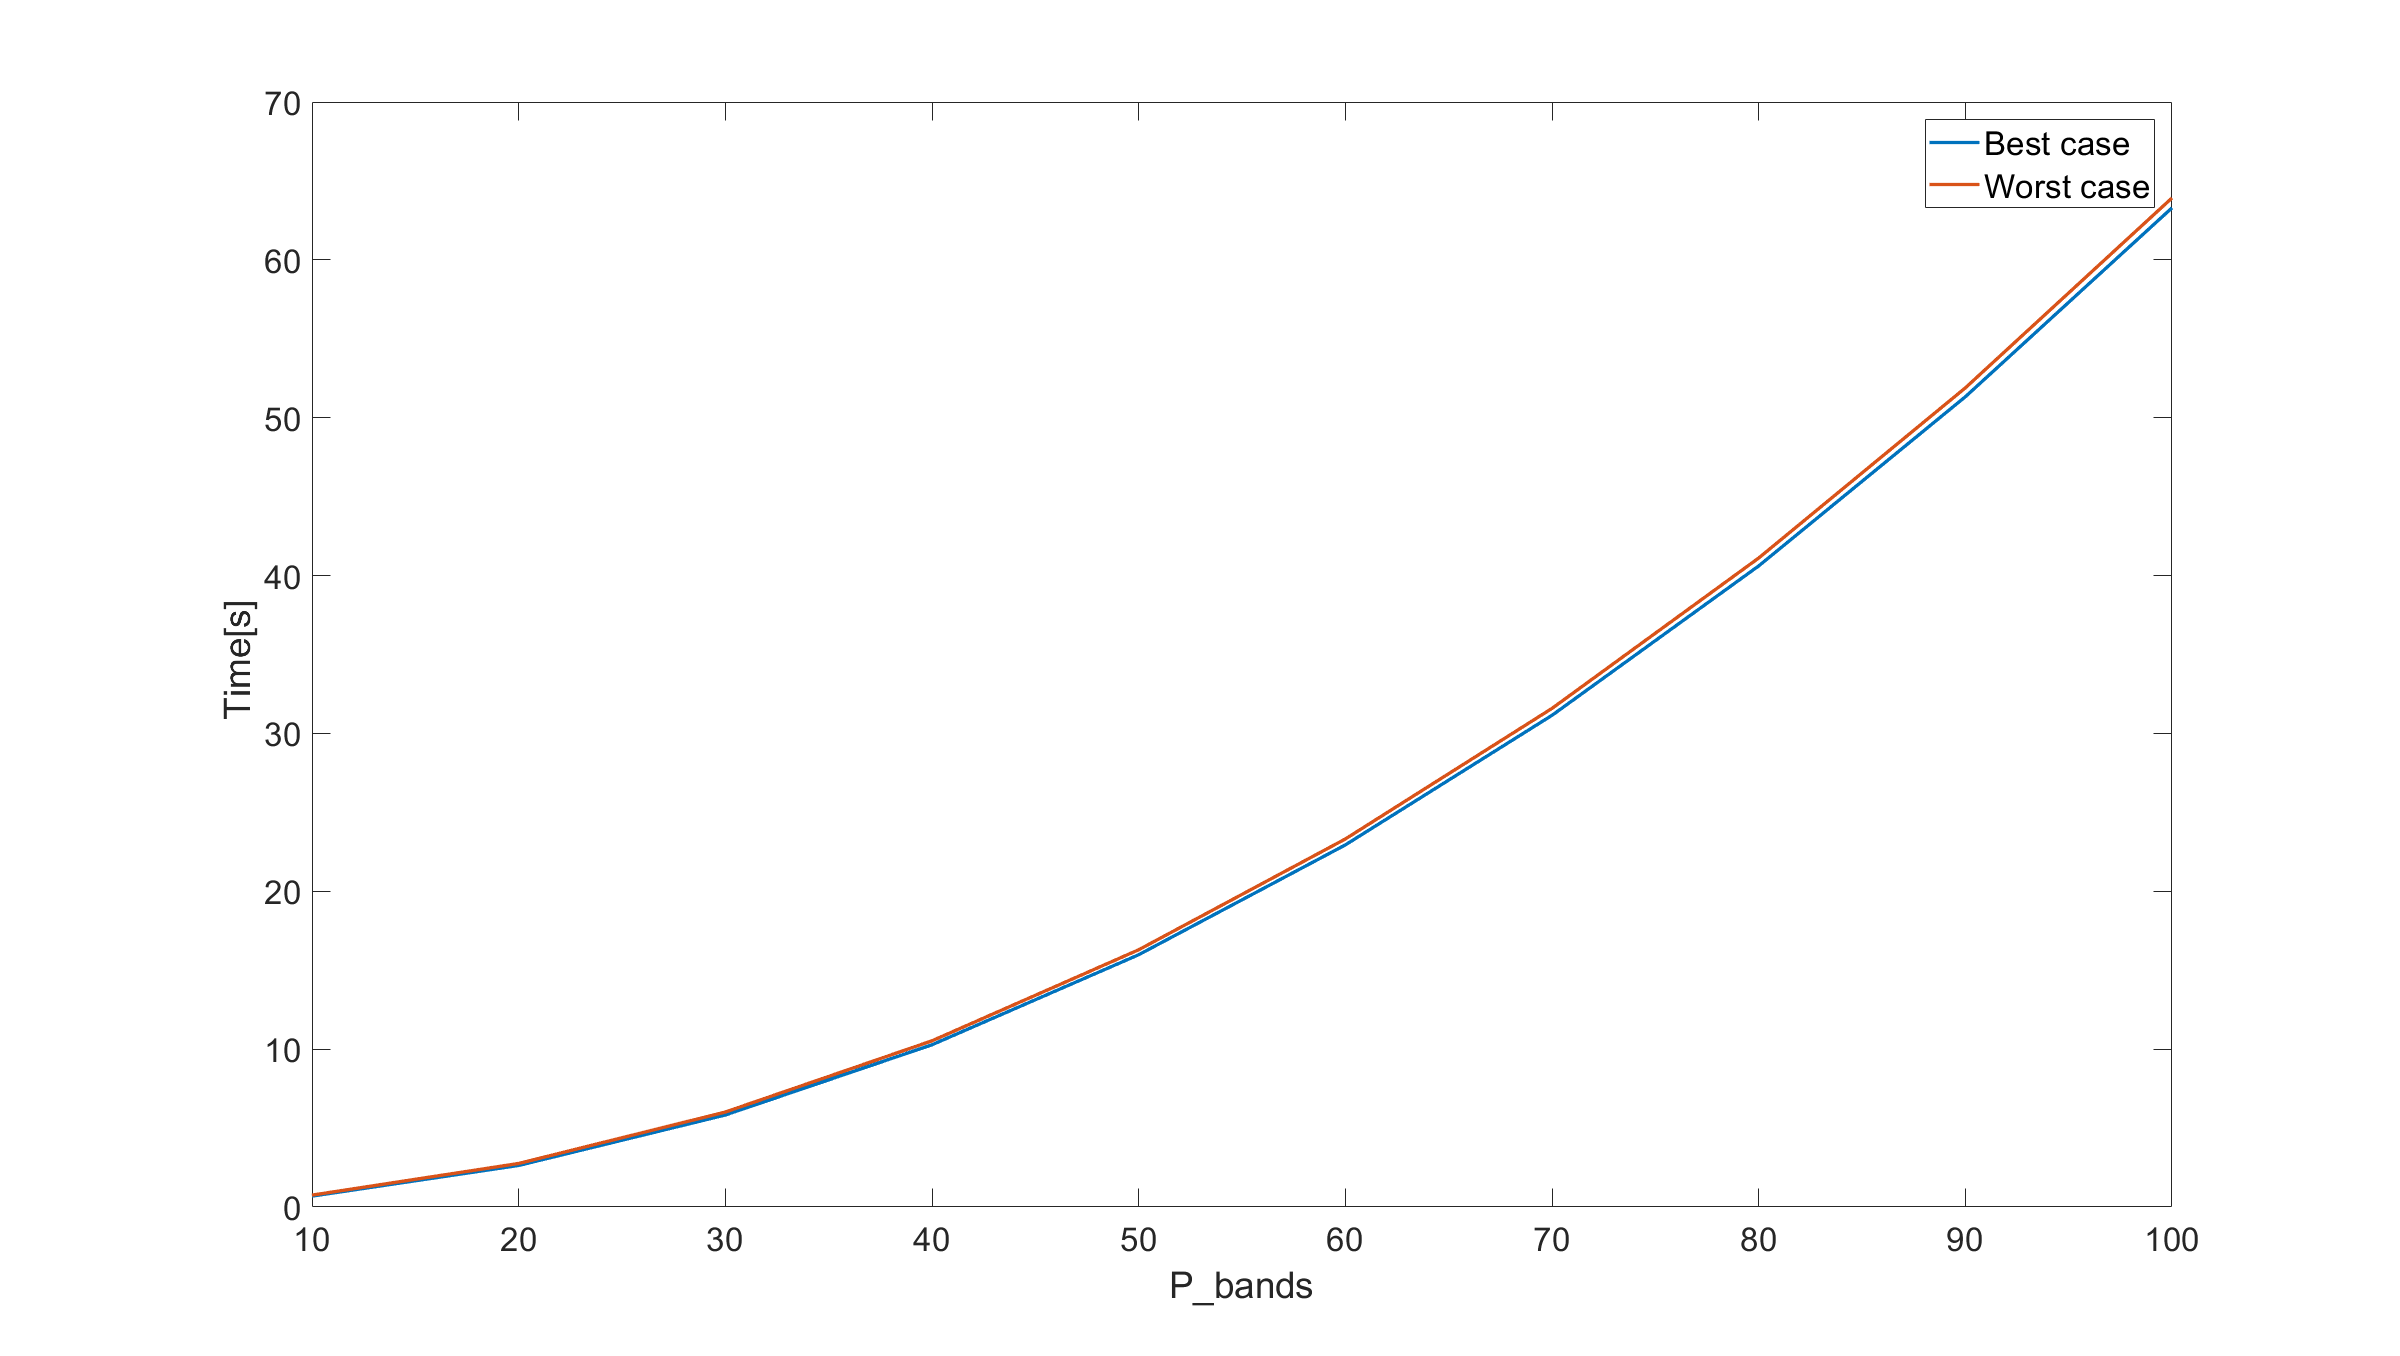
\includegraphics[scale=0.25]{images/estimated_execution_time_inverse_computation_in_seconds.png}}
  \caption{Estimated execution time for computation of $\Tilde{\textbf{R}}^{-1}(\textbf{x}_k)$ for an image of size 1088x576 in seconds. } 
  \label{fig:estimated_time_inverse}
\end{figure}
%%\subsubsection{Inverse computation}
%%Estimated execution time backward elimination:
%%\begin{equation}
%%    B=\sum_{i=1}^{i=P_{BANDS}-1} i
%%\end{equation}

\subsection{Division}
\label{sec:division_implementation}

A drawback with the Gauss-Jordan algorithm is that it uses division. Division is an operation that is computationally intensive, and requires a large amount of logic to be implemented. An early implementation of the Gauss-Jordan elimination by the author included the use of the division operator "/". This is further described in Section \ref{sec:division_operator}.\\



An approach to implement division by adaptive shifting is described in Section \ref{sec:adaptive_shifting}. 

A third approach for computing division was made. This approach utilizes LUTs to store an array containing the inverse of the divisor in the division. It is further described in Section \ref{sec:LUT_division}.\\

 The semantics used to described the division operation will be $C=B*\frac{1}{a}$ where $C,B$ and $a$ are integers in the range of s=[-$2^{Pixel\_data\_width \times 2}$-1,...$2^{Pixel\_data\_width \times 2}$-1]. %This corresponds to the inner loop operation for Last division shown in Figure \ref{fig:gauss_jordan_pseudocode}.


\subsubsection{Using division operator "/"}
\label{sec:division_operator}



%%\begin{figure}[H]
%%\centering
%%   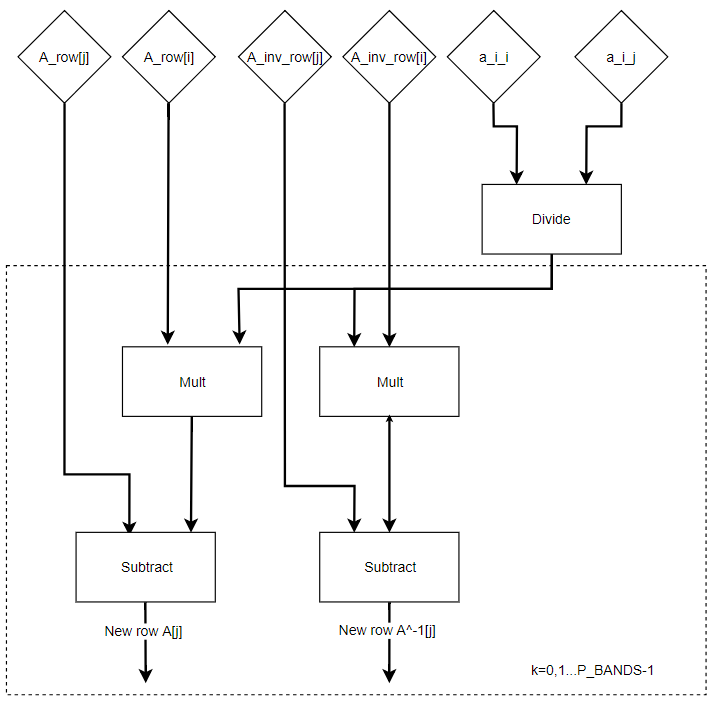
\includegraphics[scale=0.5]{images/inverse_hw/inverse_core_division_approach.PNG}
%%  \caption{Architecture of the \textbf{Elimination core} in Figure \ref{fig:top_level_inverse}, using division operator "/" for integer datatype in VHDL. $k$= $P\_BANDS$ modules marked by the dotted square is implemented in order to compute one row per clock cycle.  } 
%%  \label{fig:adaptive_shifting}
%%\end{figure}

To evaluate if division could be implemented by using the "/" operator for signed datatypes, the $\textbf{Last division}$ block was synthesized, and the worst negative slack (WNS) was used as a criteria to see if the design met the system clock target constraint of 100 MHz. 
The max frequency, $f_{max}$, is calculated by equation \ref{eq:wns}:  
\begin{equation}
f_{max}=\frac{1}{-WNS+10ns}. 
\label{eq:wns}
\end{equation}

 Results for different divisor- and- divident bit width are presented in Table \ref{tab:division_operator_wns}. The data flow for block \textbf{Last division} using the division operator can be seen in Figure \ref{fig:last_division_division_operator}.



\begin{figure}[H]
\centering
\hbox{\hspace*{-0cm}                                                           

   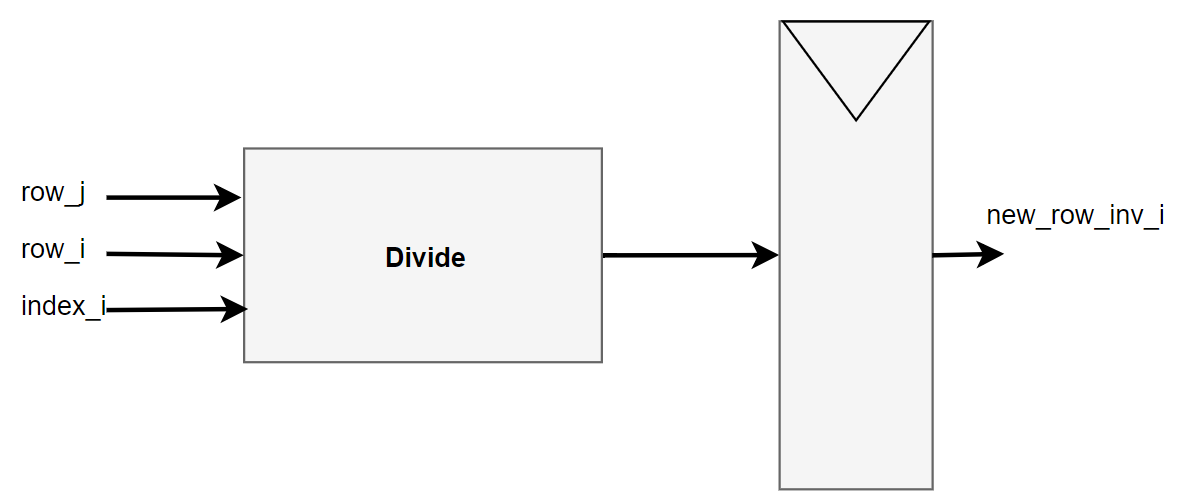
\includegraphics[scale=0.5]{images/approximate_division/last_division_division_operator.png}}
  \caption{Architecture of block \textbf{Last division} using the division operator "/" for division.   } 
  \label{fig:last_division_division_operator}
\end{figure}



%\begin{table}[H]
%    \centering
%    \begin{tabular}{c|c|c}
%    \textbf{Bit width divisor and dividend} &\textbf{Logic delay[ns]}&\textbf{Max frequency[MHz] } \\
%         32&72.498 &13.79 \\
%         13 &19.726 &50.69\\
%         10 & 16.032&62.37 \\
%         8 & 12.74&78.49 \\
%         6&9.530& 104.93\\
%         
%    \end{tabular}
%    \caption{Synthesis results for ZedBoard Zynq Evaluation and Development Kit Z7020 for \textbf{Last division} shown in Figure \ref{fig:top_level_inverse}, implementing the product $C= B*\frac{1}{A}$. Bit width for factor $B$ is 32 bit.}
%    \label{tab:division_operator_logic_delays}
%\end{table}{}
%% Insert table here, with widths and delays

\subsubsection{Adaptive shifting}
\label{sec:adaptive_shifting}
        To avoid using the division operator the adaptive shifting approach shown in \ref{fig:adaptive_shifting} has been implemented. It approximates the divisor by an adaptive number of shift operations, as the divisor is not constant. To achieve this, the most significant bit (MSB) of the divisor is first checked to evaluate if the divisor is a negative number. If it is, the divisor is negated. The block \textbf{Find MSB} finds the MSB of the unsigned divisor. In parallel, $Pixel\_Data\_Width$ $\times$ 2-1 numbers of shift-operation processes shifts the unsigned divisor by $n\_shifts$=[1,2...$Pixel\_Data\_Width$ $\times$ 2 - 1]. The remainders after shifting is sent to the \textbf{Choose best approximation} block. This block choose the best approximation depending upon the index of the MSB and the remainders after shifting. The best approximation to the divisor will be a shift operation by MSB or MSB+1 number of shifts. Each element of the row is then shifted in parallel to compute the approximate division. If the divisor is a negative number, the row is negated before outputting data to register.
        \\
       


The adaptive shifting will have an error of \textbf{FIND largest error.}. 

%\textbf{Mention the fact that r\_i\_i\_half is added before dividing. This is because of integer rounding in hardware/vivado}


\begin{figure}[H]
\centering
\hbox{\hspace*{-2cm}                                                           

   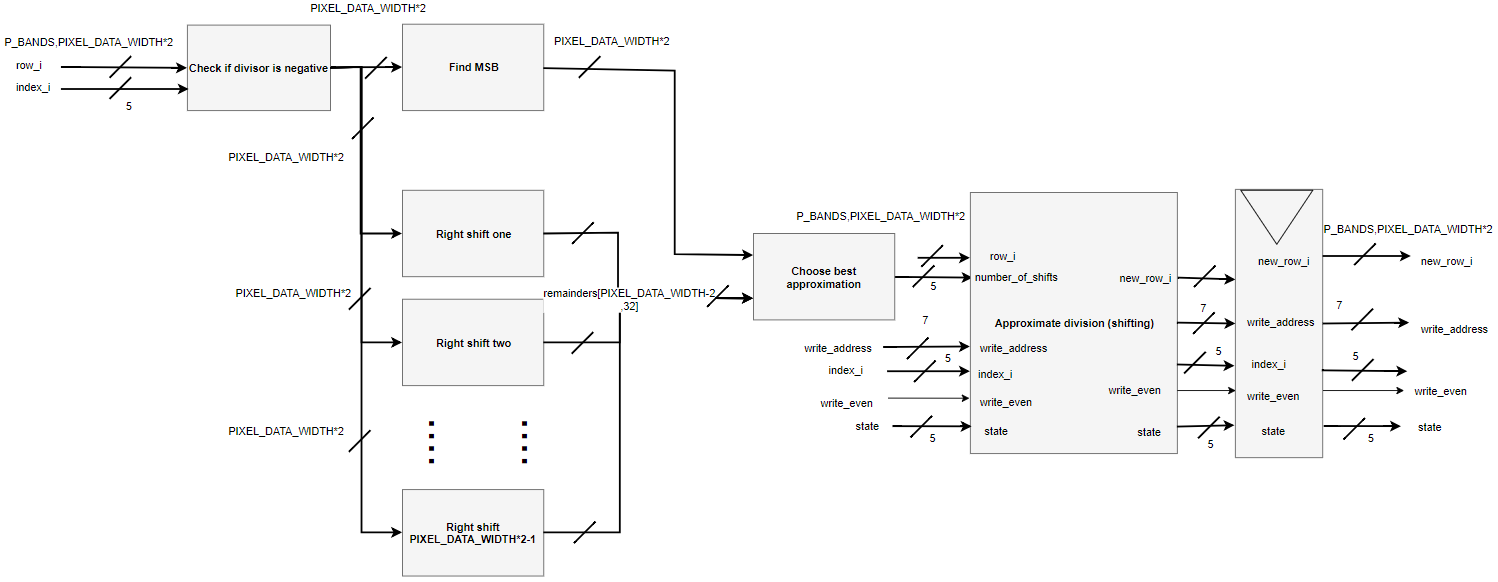
\includegraphics[scale=0.4]{images/approximate_division/last_division.PNG}}
  \caption{Architecture of block \textbf{Last division}, approaching division with an adaptive number of shifts.   } 
  \label{fig:adaptive_shifting}
\end{figure}


\subsubsection{LUT approach}
\label{sec:LUT_division}
Instead of computing the division in the operation $C= B \times \frac{1}{a}$, an approach based on the solution in \cite{cite:how_to_implement_division} was made. This approach utilizes LUTs to store the array $divisor\_inv$= \\$\frac{2^{Div\_Precision}}{a}$, where $a=[1,2...2^{Div\_Precision}]$. $Div\_Precision$ is the bit width of the divisor possible to represent with this approach. If the MSB of the divisor $a$ is at an index > $Div\_Precision$, the adaptive shifting approach is used. If not, $a$ is used as an index to look up in LUTs (number of LUTs depending upon $Div\_Precision$) storing $divisor\_inv$. $divisor\_inv(a)$ is then multiplied by $B$, which yields product $C$. $C$ is then right shifted $Div\_Precision$ spaces. This can be seen in Equation \ref{LUT_operations}.

\begin{equation} \label{LUT_operations}
\begin{split}
C= shift\_right(B \times divisor\_inv(a),Div\_Precision)
\end{split}
\end{equation}

The code for inferring LUTs for storage of $divisor\_inv$ is shown in Listing \ref{lst:lut_division}, exemplified for $Div\_Precision$=4.  

\lstinputlisting[caption={LUT division approach exemplified for Div\_Precision = 4.},label={lst:lut_division},style=customc]{code/lut_4_bit_example.vhd}

The architecture of the \textbf{Last division} block, utilizing this LUT approach, is shown in figure \ref{fig:top_last_division_lut_approach}. If $Div\_Precision$< $Pixel\_Data\_Width$ $\times$ 2, an adaptive shifting approach is added in parallel. If the MSB is located at an index > $Div\_Precision$, then the adaptive shifting approach is used.
\\

\begin{figure}[H]
\hbox{\hspace*{-2cm}                                                           

   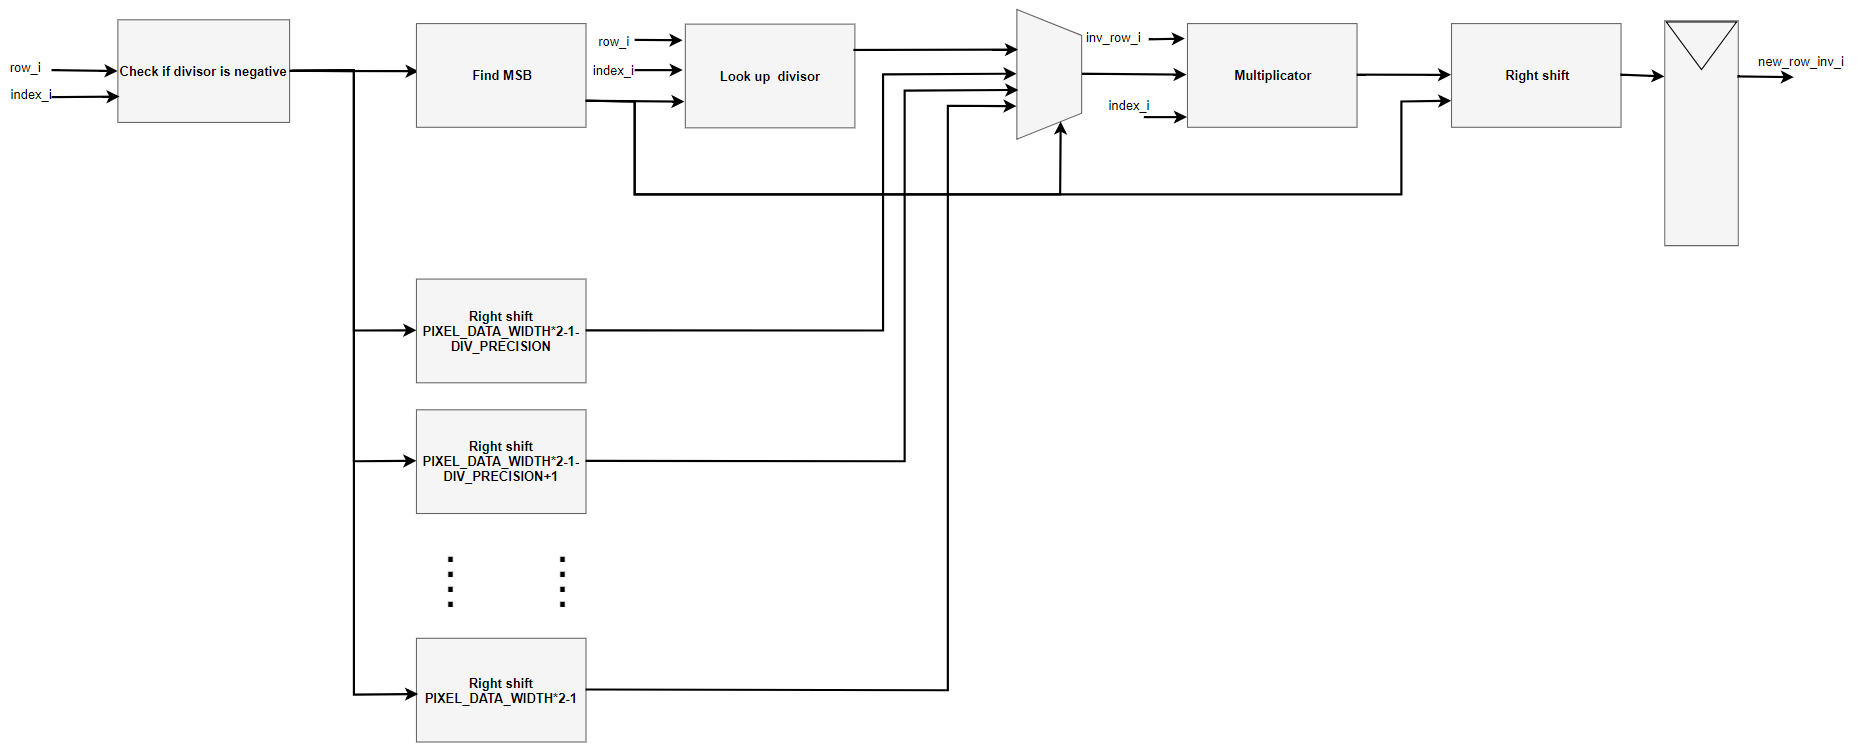
\includegraphics[scale=0.35]{images/approximate_division/top_last_division_lut_approach_dataflow.PNG}}
  \caption{Architecture of block \textbf{Last division}, computing division using the LUT approach.   } 
  \label{fig:top_last_division_lut_approach}
\end{figure}